% \RequirePackage{fix-cm}
% \RequirePackage[hyphens]{url}
\documentclass[msom,blindrev]{informs3} % current default for manuscript submission
%\documentclass[msom,nonblindrev]{informs3}


%%\OneAndAHalfSpacedXI
%%\OneAndAHalfSpacedXII % Current default line spacing
%%\DoubleSpacedXII
\DoubleSpacedXI

\makeatletter
\let\normalsize\relax
\let\@currsize\normalsize
\makeatother
\usepackage{caption}
\usepackage{subcaption}
% If hyperref is used, dvi-to-ps driver of choice must be declared as
%   an additional option to the \documentclass. For example
%\documentclass[dvips,msom]{informs3}      % if dvips is used
%\documentclass[dvipsone,msom]{informs3}   % if dvipsone is used, etc.

% Private macros here (check that there is no clash with the style)

% Natbib setup for author-year style
\usepackage{natbib}
 \bibpunct[, ]{(}{)}{,}{a}{}{,}%
 \def\bibfont{\small}%
 \def\bibsep{\smallskipamount}%
 \def\bibhang{24pt}%
 \def\newblock{\ }%
 \def\BIBand{and}%
\usepackage{multibib}
\newcites{main}{References}   % Main bibliography
\newcites{app}{Appendix References} % Appendix bibliography
\usepackage{eurosym}

%% Setup of theorem styles. Outcomment only one. 
%% Preferred default is the first option.
\TheoremsNumberedThrough     % Preferred (Theorem 1, Lemma 1, Theorem 2)
%\TheoremsNumberedByChapter  % (Theorem 1.1, Lema 1.1, Theorem 1.2)

%% Setup of the equation numbering system. Outcomment only one.
%% Preferred default is the first option.
\EquationsNumberedThrough    % Default: (1), (2), ...
%\EquationsNumberedBySection % (1.1), (1.2), ...

% In the reviewing and copyediting stage enter the manuscript number.
%\MANUSCRIPTNO{} % When the article is logged in and DOI assigned to it,
                 %   this manuscript number is no longer necessary


\usepackage{color}
\usepackage{rotating}
\usepackage{hyperref}
\usepackage{booktabs}
\usepackage{multicol}
\usepackage{caption}
\usepackage{subcaption}
\usepackage{xcolor}
\usepackage[normalem]{ulem}
\usepackage{graphicx, amsmath, amssymb, amssymb, amsfonts, enumerate, booktabs, float, adjustbox, hyperref, tikz, multirow,pgfplots,wrapfig,bm,bbm,graphicx,subcaption,enumitem,makecell,setspace}
\usepackage{url}
\usepackage[titlenumbered,ruled]{algorithm2e}

\usepackage[flushleft]{threeparttable}
\usepackage{natbib}
 \bibpunct[, ]{(}{)}{,}{a}{}{,}%
 \def\bibfont{\small}%
 \def\bibsep{\smallskipamount}%
 \def\bibhang{24pt}%
 \def\newblock{\ }%
 \def\BIBand{and}%

\newcommand{\md}[1]{\mathbb{#1}}

\allowdisplaybreaks

\usetikzlibrary{shapes.geometric, arrows}

\tikzstyle{startstop} = [rectangle, rounded corners, minimum width=3cm, minimum height=1cm,text centered, draw=black, fill=red!30]
\tikzstyle{process} = [rectangle, minimum width=3cm, minimum height=1cm, text centered, draw=black, fill=orange!30]
\tikzstyle{decision} = [diamond, minimum width=3cm, minimum height=1cm, text centered, draw=black, fill=green!30]
\tikzstyle{arrow} = [thick,->,>=stealth]

\renewcommand{\d}{\mathrm{d}}

\definecolor{myblue}{RGB}{0,51,140}
\definecolor{myred}{RGB}{126,0,0}
\definecolor{mygreen}{RGB}{0,90,0}
\definecolor{mypurple}{RGB}{142, 36, 170}
\definecolor{mygray}{RGB}{200,200,200}

\usetikzlibrary{decorations.markings}
\usetikzlibrary{decorations.pathmorphing}
\usetikzlibrary{shapes.geometric, arrows,angles,quotes}
\usetikzlibrary{arrows,decorations.pathmorphing,backgrounds,positioning,fit,matrix}
\usetikzlibrary{shapes,decorations,arrows,calc,arrows.meta,fit,positioning}
\tikzset{
	circ/.style = {draw,circle,minimum size=2.5em,inner sep=1},
	ang/.style={draw, angle eccentricity=1.5,angle radius=0.4cm}
}
 \pgfplotsset{compat=1.17} 
\newcommand*{\LargerCdot}{\raisebox{-0.25ex}{\scalebox{1.2}{$\cdot$}}}

\begin{document}

\RUNTITLE{A Framework for Cost-Benefit Analysis of COVID-19 Interventions}

\TITLE{THEMIS: A Framework for Cost-Benefit Analysis of COVID-19 Non-Pharmaceutical Interventions}
\RUNAUTHOR{Bertsimas, Li, and Soni}


\ARTICLEAUTHORS{%
\AUTHOR{Dimitris Bertsimas}
\AFF{Sloan School of Management, Massachusetts Institute of Technology, \EMAIL{dbertsim@mit.edu}}
\AUTHOR{Michael Lingzhi Li}
\AFF{Technology and Operations Management, \EMAIL{mili@hbs.edu} }
\AUTHOR{Saksham Soni}
\AFF{Sloan School of Management, Massachusetts Institute of Technology, \EMAIL{ssoni@dynideas.com}}
} 

\ABSTRACT{%
{
\linespread{0.85}\selectfont
\noindent\textbf{Problem Definition}:  Since December 2019, the COVID-19 pandemic has prompted governments worldwide to implement a wide range of non-pharmaceutical interventions (NPIs), from mass gathering restrictions to complete lockdowns. While these measures have been effective in reducing virus transmission, they also carry significant economic and humanitarian costs, including unemployment, mental health issues, and social unrest. This work aims to quantitatively assess the trade-offs between these diverse NPIs across economic and humanitarian dimensions, and to identify optimal pandemic mitigation strategies tailored to different countries, thereby aiding governments in better preparing for future pandemics.

\noindent\textbf{Methodology}: We develop THEMIS, a comprehensive data-driven counterfactual prediction framework that integrates econometric modeling, a novel epidemiological model, and data-driven cost estimates. THEMIS quantifies the impacts of various NPIs across multiple dimensions during a pandemic, enabling a robust comparison of counterfactual scenarios.


\noindent\textbf{Results}: Leveraging data from 80+ sources, we apply THEMIS to evaluate thousands of policy alternatives across the U.S., Germany, Brazil, and Spain during COVID-19. Our analysis reveals that actual policies often deviated from the efficient frontier, leading to high costs in both humanitarian and economic dimensions. Short but moderately strong restrictions (e.g., limits on gatherings, travel, and work for 6–8 weeks) generally yielded the best outcomes, whereas prolonged lockdowns imposed high costs without proportional benefits. Trade-off profiles varied significantly across regions, emphasizing the importance of tailoring policies to local economic and epidemiological conditions rather than adopting uniform strategies.

\noindent\textbf{Managerial Implications}: THEMIS provides policymakers with a powerful tool to quantify and compare the trade-offs between different NPIs, enabling more informed decision-making in pandemic response planning. By tailoring strategies to the specific socio-economic contexts of different regions, governments can optimize their responses to future pandemics, balancing economic stability with humanitarian outcomes.
}
}

\KEYWORDS{COVID-19 ; Cost-benefit Analysis ; Counterfactual Predictions ; Epidemiological modeling}

\maketitle
\section{Introduction}
\label{sec:introduction}
Starting in 2020, the world has faced one of the biggest health crises in a century: the COVID-19 pandemic. Originating in Wuhan, China, the disease, caused by the SARS-CoV-2 coronavirus, spread rapidly across the globe, resulting in the loss of over 7 million lives \citepmain{hui2020continuing}.

To curtail the spread of SARS-CoV-2 and mitigate its humanitarian impact, governments worldwide enacted unprecedented non-pharmaceutical interventions (NPIs), ranging from social distancing and mask-wearing to complete lockdowns. Despite their proven effectiveness in reducing transmission \citepmain{haug2020ranking}, these NPIs imposed significant societal costs. Restrictions on mass gatherings and travel severely impacted many industries, reducing economic output and causing mass unemployment. The travel industry alone lost \$3.8 trillion in 2020 \citepmain{wttc}, and the International Labour Organization estimates that 114 million full-time jobs were lost globally \citepmain{monitor2020covid}. Beyond economic costs, severe measures like lockdowns led to a rise in mental health issues, including depression, anxiety, and PTSD \citepmain{XIONG202055}. Researchers also raised concerns about the long-term effects of school closures on educational attainment. \citepmain{di2023impact}

This situation has sparked significant debate among the public and the scientific community about whether the benefits of these measures outweighed their costs and what better alternatives could have been used. Quantifying these costs across multiple dimensions is notoriously challenging. Moreover, identifying outcomes under alternative policies requires understanding the impact of different NPIs on the spread of COVID-19 and simulating counterfactual scenarios.

Given these challenges, it is unsurprising that, despite significant global interest, there remains a lack of comprehensive, data-driven analyses that evaluate pandemic policies across both economic and health dimensions. Most prior cost-benefit studies have either focused on assessing the trade-offs of policies as they were implemented \citepmain{broughel2021benefits, cutler2020covid} or examined the economic impact of specific NPIs, often emphasizing direct GDP effects \citepmain{layard2020release, shlomai2021modeling, rowthorn2020cost, miles2021stay, gros2020great, zhao2021disease}. In contrast, we take a retrospective, global approach, leveraging empirical data from the COVID-19 pandemic to develop THEMIS—a data-driven framework designed for comprehensive cost-benefit analysis. THEMIS enables the evaluation of both actual policy sequences and a broad set of counterfactual alternatives, providing a structured approach to understanding the trade-offs inherent in pandemic response strategies. We name our framework after THEMIS, the Greek goddess of law and balance, to reflect its goal of systematically weighing economic and humanitarian considerations in policymaking.

To simulate the pandemic under different NPI sequences, we employ the policy-driven compartmental epidemiological model DELPHI. DELPHI extends classical compartmental models to capture key features of the COVID-19 pandemic, such as underdetection due to limited testing, governmental and societal responses, and declining mortality rates \citepmain{li:20}. Since April 2020, DELPHI has been applied to over 200 countries and regions, producing country and state-level predictions. DELPHI forecasts have been incorporated into the central ensemble at the CDC and used by various organizations for pandemic planning.

In assessing the costs associated with the pandemic under various policy scenarios, we focus on both economic and humanitarian dimensions, following the broad categorizations established in previous research \citepmain{cutler2020covid}. We emphasize directly measurable costs in both categories. Humanitarian costs include direct consequences of COVID-19 infections, such as mortality, hospitalization, long-term health impairments, and mental health challenges. Economic costs encompass reductions in output, increased unemployment, and the associated economic burdens. We acknowledge the complexity and multitude of costs resulting from COVID-19, recognizing that any attempt to quantify these is necessarily partial. A detailed discussion of why certain significant costs were not included in our analysis is provided in Section \ref{sec:discussion}. Each cost item is modeled based on the most recent and relevant studies, and a detailed discussion on the selection and verification of sources is contained in Appendix \ref{app:region_specific_params}.

To demonstrate the wide applicability of the THEMIS framework, we implemented it for Germany, the United States, Spain, and Brazil, using the latest economic and health data (see Appendix \ref{app:region_specific_params} for sources). We investigated the optimal 3-month NPI sequence starting on March 15, 2020, when governments were considering responses to the growing pandemic.

Our simulation results yield three main insights. First, the effectiveness of NPIs varies significantly across regions, emphasizing the need for tailored interventions rather than uniform strategies. In high-density areas, both extreme and lenient policies resulted in high economic costs, making moderate interventions more effective. Second, while NPIs can significantly reduce humanitarian costs, overly stringent lockdowns do not always yield proportional benefits and can impose unnecessary economic and mental health burdens. Third, timing plays a crucial role—early intervention can drastically reduce total costs, but in some regions, delays in response meant that even the most stringent measures would have had limited impact.

In summary, this paper contributes by formulating a novel quantitative model, THEMIS, for conducting cost-benefit analyses of COVID-19 NPIs and provides practical insights from applying the THEMIS model to various countries. The THEMIS codebase is open-source and available at \url{https://github.com/COVIDAnalytics/THEMIS}, facilitating its application to other regions.


\section{THEMIS Framework Formulation}
\label{sec:model}

The schematic for the THEMIS Framework is shown in Figure \ref{fig:data_flowchart}. THEMIS starts with the input of a policy $\bm{P}= (\bm{I},\bm{T})$, which we formally define as a combination of $k$ NPIs $\bm{I}=(i_0,\cdots,i_{k-1})$ and $(k+1)$ implementation times $\bm{T}=(t_0,t_1,\cdots,t_k)$ where $t_0<t_1<\cdots<t_k$. The policy is implemented such that each NPI $i_l$, $l \in \{0,\cdots,k-1\}$ is effective between $[t_l,t_{l+1}]$, and is selected from a set of possible NPIs $\mathcal{I}$. For example, the policy $\bm{P}$ with:
\begin{align*}
    \bm{I} &= (\text{Lockdown}, \text{Social Distancing}, \text{No Restrictions})\\
    \bm{T} &=(2020.03.01, 2020.04.01, 2020.05.01, 2020.06.01)
\end{align*}
%% It would be good to add a table of all the NPIs we are considering and their description if needed
represents a policy from March 1st, 2020 to June 1st, 2020 with the stages as outlined in Table \ref{tab:example_policy}. We note that this structure is general and all policies implemented in the COVID-19 pandemic can be written in such structure, given a sufficiently large set of $\mathcal{I}$. For simplicity only, we would assume throughout this paper that $t_l$ for $l\in \{0,\cdots,k\}$ has units of days. 


\begin{table}[h!]
\centering
\resizebox{0.5\textwidth}{!}{
\begin{tabular}{|c|c|c|}
\hline
     \textbf{Policy Start Date}& \textbf{Policy End Date} & \textbf{Policy}  \\\hline
     March 1st, 2020 & April 1st, 2020 & Lockdown\\
     April 1st, 2020 & May 1st, 2020 & Social Distancing\\     
     May 1st, 2020 & June 1st, 2020 & No Restrictions\\\hline
\end{tabular}
}
\caption{Example Policy}
\label{tab:example_policy}
\end{table}
The goal of THEMIS is to quantify the total cost of a given policy $\bm{P}$ for a specific region, incorporating region-specific data $\bm{R}$. This total cost, denoted as $c_R(\bm{P})$, is evaluated over the policy implementation period $t \in [t_0,t_k]$. As illustrated in Figure \ref{fig:data_flowchart}, the first step in this process is to simulate the evolution of the epidemic states $\bm{M}$ under policy $\bm{P}$ using the DELPHI epidemiological model, yielding $\bm{M} = f(\bm{R},\bm{P})$. We then compute the resulting costs of the epidemic by considering both $\bm{P}$ and $\bm{M}$.

To ensure a structured cost analysis, we classify costs into two broad categories—economic and humanitarian—following \cite{cutler2020covid}. Within the humanitarian cost category, we consider both physical health costs (loss of life $c_{R,LL}$ and hospitalizations $c_{R,H}$) and mental health costs $c_{R,M}$. For economic costs, we capture both the direct economic impact of the epidemic and NPIs in terms of GDP losses $c_{R,Y}$, as well as the indirect costs due to reduced well-being caused by unemployment $c_{R,U}$. 

The total cost of a policy $\bm{P}$ is then computed as:
\[c_R=c_{R,U} + c_{R,Y} + c_{R,LL} + c_{R,H} + c_{R,M},\]
where we suppress the dependence on the policy $\bm{P}$ when it is clear. The following subsections describe the detail construction of each model ($f$,$c_{R,U}$,$c_{R,Y}$,$c_{R,LL}$,$c_{R,H}$,$c_{R,M}$). 

\begin{figure*}[h!]
\centering
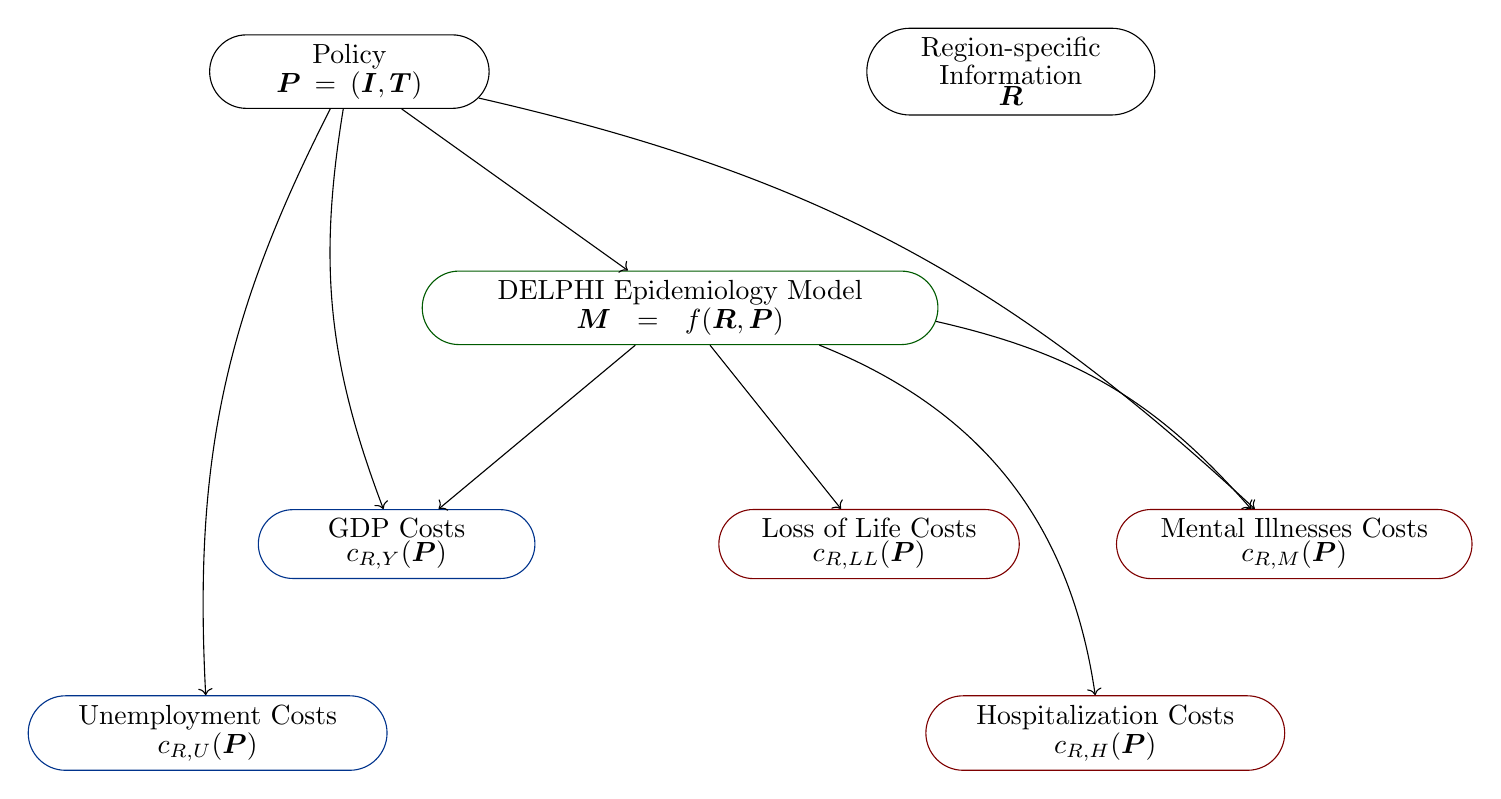
\begin{tikzpicture}[scale=0.6]
\linespread{0.5}\selectfont
\node[rounded rectangle, draw=black, text width=3cm, align=center] (Policy) at (3, 12) {Policy\\ $\bm{P}=(\bm{I},\bm{T})$};
\node[rounded rectangle, draw=black, text width=3cm, align=center] (Region) at (17, 12) {Region-specific Information\\ $\bm{R}$};
\node[rounded rectangle, draw=mygreen, text width=6cm, align=center] (DELPHI) at (10, 7) {DELPHI Epidemiology Model\\ $\bm{M}=f(\bm{R},\bm{P})$};
\node[rounded rectangle, draw=myblue, text width=4cm, align=center] (Unemployment) at (0, -2) {Unemployment Costs \\$c_{R,U}(\bm{P})$};
\node[rounded rectangle, draw=myblue, text width=3cm, align=center] (GDP) at (4, 2) {GDP Costs \\$c_{R,Y}(\bm{P})$};
\node[rounded rectangle, draw=myred, text width=3.3cm, align=center] (Mortality) at (14, 2) {Loss of Life Costs\\$c_{R,LL}(\bm{P}) $};
\node[rounded rectangle, draw=myred, text width=4cm, align=center] (Hospitalization) at (19, -2) {Hospitalization Costs\\$c_{R,H}(\bm{P})$};
\node[rounded rectangle, draw=myred, text width=4cm, align=center] (Mental) at (23, 2) {Mental Illnesses Costs\\$c_{R,M}(\bm{P})$};
\draw[->] (Policy)--(DELPHI);
\draw[->] (Policy) to [bend left=15] (Mental);
\draw[->] (Policy) to [bend right=15] (Unemployment);
\draw[->] (Policy) to [bend right=15] (GDP);
\draw[->] (DELPHI) to [bend left=18] (Mental);
\draw[->] (DELPHI) --(GDP);
\draw[->] (DELPHI) --(Mortality);
\draw[->] (DELPHI) to [bend left=30] (Hospitalization);
\end{tikzpicture}
\caption{THEMIS Schematic. Here we ignore the arrows from $\bm{R}$ to every module for simplicity.}
\label{fig:data_flowchart}
\end{figure*}
\subsection{The DELPHI model $f$: Forecasting the dynamics of the COVID-19 pandemic}
\label{subsec:delphi}
DELPHI is a policy-driven compartmental epidemiological model that extends the widely used SEIR model to account for effects specific to the COVID-19 pandemic.  The model is governed deterministically by a system of ordinary differential equations (ODEs) involving 11 states: susceptible ($M^S$), exposed ($M^E$), infectious ($M^I$), undetected cases who will recover ($M^{UR}$) or die ($M^{UD}$), detected hospitalized cases who will recover ($M^{HR}$) or die ($M^{HD}$), detected quarantined cases who will recover ($M^{QR}$) or die ($M^{QD}$), recovered ($M^{R}$) and deceased ($M^{D}$). Within the hospitalized states ($M^{HR},M^{UD}$), there are also helper states to govern patients that are in the ICU ($M^{IC}$) and patients who are ventilated ($M^{V}$). Since its conception in late March 2020, it has been successfully applied to more than 210 countries and regions worldwide with high accuracy, and is utilized by organizations including the Hartford Hospital system for pandemic planning. \citepmain{li:20}

DELPHI differs from other COVID-19 forecasting models \citepmain[see, e.g.][]{kissler:20} by capturing three key elements of the pandemic: 
\begin{itemize}
    \item \textbf{Under-detection}: Many cases remain undetected due to limited testing, asymptomatic carriers, and detection errors. Ignoring them would underestimate the scale of the pandemic. The DELPHI model captures them through the $M^{UR}$ and $M^{UD}$ states.
    \item \textbf{Governmental and societal response}: Social distancing policies limit the spread of the virus. Ignoring them would overestimate the scale of the pandemic. However, if restrictions are lifted prematurely, a resurgence may occur. We define a governmental and societal response function $\gamma(t)$, which modulates the infection rate and is parameterized as follows: 
    \begin{equation}
        \gamma(t)=1 + \frac{2}{\pi}\arctan\left(\frac{-(t-t_\text{int})}{\kappa}\right) + c\exp\left(-\frac{(t-t_\text{jump})^2}{2\sigma^2}\right). \label{eq:gamma}
    \end{equation}
    This parameterization encompasses four phases (Figure~\ref{fig:response_function}). In Phase I, most activities continue normally as people adjust their behaviors. This is followed by a sharp decline in the infection rate during Phase II as the policies get implemented. The parameters $t_{\text{int}}$ and $\kappa$ can be interpreted as the start time and the strength of this response. In Phase III, the decline in the infection rate reaches saturation. The epidemic then experiences a resurgence of magnitude $c$ in Phase IV, due to relaxations in governmental restrictions and in social behaviors. This is counteracted at time $t_{\text{jump}}$, when restrictions are re-implemented, with $\sigma$ controlling the duration of this second wave.
\begin{figure*}[ht!]
    \centering
    \includegraphics[width=0.8\textwidth]{images/response_function.png}
    \caption{Governmental and societal response function $\gamma(t)$ ($\kappa=5$, $t_{\text{int}}=10$, $c=1$, $t_{\text{jump}}=25$ and $\sigma=2$).}
    \label{fig:response_function}
\end{figure*}
    \item \textbf{Declining mortality rates}: The mortality rate of COVID-19 has been declining through the pandemic, due to a better detection of mild cases, enhanced care for COVID-19 patients, and other factors. We model the mortality rate as a monotonically decreasing function of time:
    \begin{align}
        m(t) &= \left(m_0 - m_{\min}\right)\left(1 + \frac{2}{\pi}\arctan\left(-r_m t\right)\right) \nonumber+ m_{\min}, \label{eq:mortality}
    \end{align}
    where $m_0$ is the initial mortality rate, $m_{\min}$ is the minimum mortality rate and $r_m$ is a decay rate. 
\end{itemize}

Ultimately, DELPHI involves 16 parameters that define the transition rates between the 11 states. We calibrate 7 of them from a database on clinical outcomes \citepmain{bertsimas:20}. Using non-linear optimization, we estimate the other 9 parameters from historical data on the number of cases and deaths in each region. We provide the full mathematical formulation of the DELPHI model and its fitting procedure in Appendix~\ref{app:delphi_fitting_procedure}. 

We utilize the DELPHI model to provide THEMIS with a highly accurate epidemiological model that responds to changes in policy. \citemain{li:20} in particular shows that the two-week out-of-sample median absolute percentage error on predicting cases and deaths across 200 geographical areas is $6\%$. The key feature of DELPHI that is specifically relevant to THEMIS is that within the region $R$, the rate of people being exposed to the virus and leaving the susceptible state ($M^{S}$) is policy-driven, and governed by the following differential equation:
\begin{equation}
    \frac{\d M^{S}}{\d t} = -\alpha_R \gamma_R(t) M^S(t)M^I_R(t).\label{eq:S}
\end{equation}
Here $\alpha_R$ is the fitted natural infection rate of the epidemic in the region, while $\gamma_R(t)$ is the fitted, time-varying, policy dependent, reduction of such infection rate in the region for the actual implemented policy. The functional form of $\gamma_R(t)$ normalizes the range of $\gamma_R(t)$ to $[0,2]$ so that $\alpha_R$ and $\gamma_R(t)$ can be individually identified.

To simulate the pandemic for a hypothetical policy scenario $\bm{P}=(\bm{I},\bm{T})$, we will thus create a counterfactual infection rate reduction curve $\gamma_R^P(t)$ through historical data. 

We first calculate the average reduction of natural infection rate for that region $R$ under each possible policy $i$, $\gamma_{R,i}$. Many regions only ever implemented a subset of policies in $\mathcal{I}$, which we denote $\mathcal{I}_R$. To formulate a general relationship that allows us to calculate $\gamma_{R,i}$ for all $R$ and $i$, we assume that
$\gamma_{R,i}$ follows:
\begin{equation}
    \gamma_{R,i} = k_R \gamma_i + \epsilon_R, \label{eq:uobsgamma}
\end{equation}
where $\epsilon_R$ represents independent zero-mean noise. The term $\gamma_i$ is the global average reduction of the natural infection rate under policy $i$, given by:
\begin{equation}
    \gamma_i = \frac{\sum_{R} \sum_{t \in \mathcal{D}_{R,i}} \gamma_{R}(t)}{\sum_{R} |\mathcal{D}_{R,i}|}.
\end{equation}
This formulation assumes that the multiplicative difference between the global and regional effects is uniform across policies. Such an assumption is reasonable, as the primary factors influencing indivudal country difference—such as societal behavior, infrastructure, and healthcare capacity—tend to not vary significantly with the type of NPI implemented. In this framework, $k_R$ thus represents the regional adjustment factor that aligns the global estimate $\gamma_i$ with the local policy effect $\gamma_{R,i}$. 

For a policy $i \in \mathcal{I}_R$ that was observed for region $R$, we calculate $\gamma_{R,i}$ by taking an average of the value of $\gamma_{R}(t)$ over the total number of days when $i$ was implemented in region $R$:
\begin{equation}
    \gamma_{R,i} = \frac{\sum_{t \in \mathcal{D}_{R,i}} \gamma_{R}(t)}{|\mathcal{D}_{R,i}|}, \qquad  i \in \mathcal{I}_R,
    \label{eq:obsgamma}
\end{equation}
where $\mathcal{D}_{R,i}$ is the set of days when $i$ was implemented in region $R$. Then to estimate the effect $\gamma_{R,i}$ for a policy $i \not \in \mathcal{I}_R$ that has not been observed in region $R$, We estimate $k_R$ by minimizing the mean-squared error on the observed pairs $(\gamma_{R,i},\gamma_i)$. Specifically, the optimal solution for $k_R$ solves the following optimization problem: 
\begin{equation}
    \min_{k} \sum_{t=1}^T \left(\frac{\gamma_R(t)}{\sum_j \mathbf{1}\{t \in \mathcal{D}_{R,i}\} \gamma_i} - k\right)^2, \label{eq:equivalent}
\end{equation}
which yields the solution:
\begin{equation}
    \hat{k}_R = \sum_{j \in \mathcal{I}_R} 
    \frac{|N_{R,j}|}{\sum_j |N_{R,j}|} \frac{ \gamma_{R,j}}{\gamma_{j}}.
\end{equation}
This estimation procedure also facilitates the quantification of uncertainty in $k_R$. Specifically, we define the standard deviation of the regional adjustment factor as:
\begin{equation}
    \sigma( \hat{k}_R) = \sqrt{\frac{1}{T} \sum_{t=1}^T \left(\frac{\gamma_R(t)}{\sum_j \mathbf{1}\{t \in \mathcal{D}_{R,i}\} \gamma_i} - k_R\right)^2}. \label{eq:uncertainty}
\end{equation}
The metric $\sigma( \hat{k}_R)$ provides a measure of variance in the regional adjustment factor based on historical data. A low variance suggests that $ \hat{k}_R$ is stable and reliable among policies implemented within the region, increasing confidence in its use for estimating the effect of unobserved policies.

For any $i \not \in \mathcal{I}_R$, we impute the regional-specific policy effect $\gamma_{R,i}$ using the estimated regional adjustment factor:
\begin{equation}
    \gamma_{R,i} =  \hat{k}_R \gamma_i. \label{eq:uobsgamma}
\end{equation}

% Old explanation for linear regression
% Then, for any region $R$,for a NPI $i_{uobs} \in \mathcal{I}$ that were not historically implemented in region $R$, we perform a linear regression between the global and region-specific reduction factors ($\gamma_{i_{obs}}$, $\gamma_{R,i_{obs}}$) on policies that are observed, and utilize the imputed value as the region-specific reduction factor $\gamma_{R,i_{uobs}}$, as shown in Figure \ref{fig:linear_interpolation}. 
% Saksham you can probably expand on this and make some of these sentences more precise

% \begin{figure}[t!]
% \centering
% 		\begin{tikzpicture}[scale=2.5]
% 	\draw[->] (0,0) -- (2.5,0) coordinate (x axis)  node[right, black]{\begin{tabular}{c}$\gamma_i$ \end{tabular}};
% 	\draw[->] (0,0) -- (0,2.5) coordinate (y axis) node[above, black]{$\gamma_{R,i}$};
% 	\node[circle,fill=black,inner sep=0pt,minimum size=3pt] (a) at (0.4,0.4) {};
% 	\node[circle,fill=black,inner sep=0pt,minimum size=3pt] (ax) at (0.4,0) {};	
% 	\node[circle,fill=black,inner sep=0pt,minimum size=3pt] (ay) at (0,0.4) {};	
%     \draw[dashed,-] (a) -- (ax);
%     \draw[dashed,-] (a) -- (ay);
% 	\node[below=0.1cm of ax] {$\gamma_{i_{obs,1}}$};
% 	\node[left=0.1cm of ay] {$\gamma_{R,i_{obs,1}}$};
% 	\node[circle,fill=black,inner sep=0pt,minimum size=3pt] (b) at (2.0,2.0) {};
% 	\node[circle,fill=black,inner sep=0pt,minimum size=3pt] (bx) at (2.0,0) {};	
% 	\node[circle,fill=black,inner sep=0pt,minimum size=3pt] (by) at (0,2.0) {};	
% 	\draw[dashed,-] (b) -- (bx);
% 	\draw[dashed,-] (b) -- (by);
% 	\node[below=0.1cm of bx] {$\gamma_{i_{obs,2}}$};
% 	\node[left=0.1cm of by] {$\gamma_{R,i_{obs,2}}$};
% 	\draw[black,thick,-] (a) --  (b);	
% 	\node[circle,fill=blue,inner sep=0pt,minimum size=3pt] (c) at (1.2,1.2) {};
% 	\node[circle,fill=blue,inner sep=0pt,minimum size=3pt] (cx) at (1.2,0) {};	
% 	\node[circle,fill=red,inner sep=0pt,minimum size=3pt] (cy) at (0,1.2) {};		
% 	\draw[dashed,->, blue] (cx) -- (c);
% 	\draw[dashed,->, blue] (c) -- (cy);
% 	\node[below=0.1cm of cx, blue] {$\gamma_{i_{uobs}}$};
% 	\node[left=0.1cm of cy, red] {$\gamma_{R,i_{uobs}}$};	
% 	\end{tikzpicture}
% 	\caption{A linear interpolation procedure to impute the impact of policies on the infection rate $\gamma_{R,i_{uobs}}$ that were not implemented in region $R$, using the global estimated impact $\gamma_i$.} \label{fig:linear_interpolation}
% \end{figure}

Then, for the hypothetical policy $\bm{P}=(\bm{I},\bm{T})$, we define $\gamma_R^P(t)$ as a piecewise constant function of the region-specific reduction factors:
\begin{equation}
    \gamma_R^P(t)=\begin{cases}
    \gamma_{R,i_0} & t_0\leq t<t_1\\
    \gamma_{R,i_1} & t_1\leq t<t_2\\ 
    \vdots & \vdots \\
    \gamma_{R,i_{k-1}} & t_{k-1}\leq t<t_k\\ 
    \end{cases}
\end{equation}
Intuitively, we are assuming that each NPI has a region-specific constant reduction $\gamma_{R,i}$ on the infection rate during its duration of application. Thus, by changing the policy $\bm{P}$, the evolution of the pandemic $\bm{M}$ would be different. 


\subsection{Humanitarian Cost Models}
\label{subsec:humanitarian_cost}
The first major category of cost during the pandemic is the humanitarian cost. This includes not just the physical health component of hospitalization and deaths in the COVID-19 pandemic, but also the impact on mental health. The NPIs induce isolation and confinement, leading to increased mental illnesses, while healthcare workers on the COVID-19 front-line experience PTSD \citepmain{liu2020factors,carmassi2020ptsd}. We develop models for these components of humanitarian cost below. 
%% Michael: TODO


\subsubsection*{Cost due to COVID-19 Loss of Life}

COVID-19 causes loss of life through two primary mechanisms: a direct loss-of-life due to premature mortality, and an indirect loss-of-life due to long COVID. For the direct loss-of-life costs, we consider the total value of the lost life years due to the premature mortality. This allows us to adjust for the skew in COVID-19 mortality that is predominantly concentrated in the elder age group. Specifically, we assume that each individual of age $u$ who died from COVID-19 would have otherwise on average lived for $l_R(u)$ life years, where $l_R(u)$ is the expected remaining life expectancy at age $u$ for the population in the region $R$ under consideration. Then, we denote the Probability Density Function (PDF) of age in COVID-19 deaths in that region as $f_R(u)$. Using $f_R(u)$ and $l_R(u)$, we can calculate the expected lost life-years for each COVID-19 death as:
\begin{equation}
    \int_0^{U} l_R(u)f_R(u) \; \d u,
\end{equation}
where $U$ is a specified age upper bound. Then, we calculate the total cost of life years lost using the total number of deaths in the epidemic $M^D$ and the value of a statistical life-year (VSLY) $c_{R,VSLY}$:
\begin{equation}
    c_{R,D}= c_{R,VSLY} \times M^D \times  \int_0^{U} l_R(u)f_R(u) \; \d u
\end{equation}

Another mechanism of loss-of-life results from Long COVID. Long COVID refers to the chronic symptoms experienced by $p_{LC}$ of COVID-infected individuals that remain after the acute infection is cleared. These chronic symptoms continue for $T_{LC}$ years and reduces life utility by $\Delta l$. Therefore, the total indirect loss-of-life due to loss of utility from Long COVID can be calculated as:
\[c_{R,LC} = c_{R,VSLY} \times M^R \times p_{LC} \times T_{LC} \times \Delta l,\]
where $M^R$ is the total number of people who recovered from COVID-19. The total cost of loss of life can be summarized as:
\[c_{R,LL} = c_{R,D} + c_{R,LC}\]
\subsubsection*{Cost of COVID-19 Hospitalizations}
Our calculation of the cost of COVID-19 hospitalizations separates into three categories: general hospitalizations, Intensive Care Unit (ICU) hospitalizations, and ventilated hospitalizations. This separation is natural due to the large differences in both the length and cost of treatment across the three categories, of which the DELPHI epidemiological model takes into account. Therefore, we can extract the total number of hospitalization-days in each category from the DELPHI simulated pandemic $\bm{M}$ as $M^H_R, M^I_R, M^V_R$ respectively. Then, denoting the daily treatment cost in each category as $c^D_{R,H}, c^D_{R,I}, c^D_{R,V}$, the cost of COVID-19 hospitalizations can be written as:
\begin{equation}
    c_{R,H}=c^D_{R,H}M^H_R,+c^D_{R,I} M^I_R+c^D_{R,V} M^V_R
\end{equation}

\subsubsection*{Cost of Mental Illnesses}
For mental illnesses, we focus on the effects of the pandemic and policies on post-traumatic stress disorder (PTSD) and depression, highlighted by multiple studies as the leading mental health issues arising in the pandemic \citepmain[e.g.][]{pfefferbaum2020mental,usher2020covid,zhong2021mental}. Specifically, there has been a sharp increase in PTSD among healthcare workers and hospitalized COVID-19 patients, while the general population experiences a significant increase in rate of clinical depression due to isolation caused by containment policies \citepmain{liu2020factors,carmassi2020ptsd}. We would consider both these effects in our calculations. Specifically, we write $N_R$ for the total population in the region, and $N_{R,H}$ as the total number of health workers. 

To calculate the cost of depression, we make a few practical assumptions. First, we assume that the increase in clinical depression is proportional to the degree of severity of the NPI, where severity is measured by $1-\gamma_{R,i}$, the percentage reduction of infection rate in region $R$ under NPI $i$. Denote the increase in prevalence of clinical depression under the most severe NPI $i^*$ in the general population as $\Delta r_{R, Dep}$ and the total general population as $N$. $\Delta r_{R, Dep}$ is estimated through population surveys with sources included in Appendix \ref{app:region_specific_params}. Then, if we write the daily cost of depression as $c_{R, Dep}$, the total cost of depression can be written as:
\begin{equation}
    c_{R, Dep} \times N_R\Delta r_{R, Dep} \times \sum_{l=1}^k (t_l-t_{l-1}) \frac{1-\gamma_{R,i_l}}{1-\gamma_{R,i^*}}
\end{equation}
Compared to depression induced by the containment policies, PTSD due to either COVID-19 hospitalization or working closely with severe COVID-19 patients can be more persistent \citepmain{carmassi2020ptsd}. We assume that PTSD due to effects of COVID-19 continue for $T_{PTSD}=1$ year \citepmain{serra2022post}. We denote the increase in prevalence of PTSD among the susceptible population as $\Delta r_{R,PTSD}$. Then the total cost of PTSD can be written as:
\begin{equation}
    c_{R,PTSD} \times (N_{R,H}+E_{R,H}+E_{R,V}+E_{R,I})\Delta r_{R,PTSD} \times T_{PTSD}
\end{equation}
Therefore, the total cost of mental illnesses is:
\begin{align}
    c_{R,M} &=c_{R,Dep} \times N_R\Delta r_{R,Dep} \times \sum_{l=1}^k (t_l-t_{l-1}) \frac{1-\gamma_{R,i_l}}{1-\gamma_{R,i^*}}\nonumber \\&+c_{R,PTSD} \times (N_{R,H}+E_{R,H}+E_{R,V}+E_{R,I})\Delta r_{R,PTSD} \times T_{PTSD}
\end{align}




\subsection{Economic Cost Models}
\label{subsec:economic_cost}
Beyond the humanitarian impact, the COVID-19 pandemic created an outsized shock to the economy. The effect of the pandemic, and the NPIs aimed to slow the spread created large economic consequences that goes beyond the direct GDP impact. In particular, the reduced output triggered massive unemployment, which carries significant costs on its own. Therefore, in this category, we would consider both the direct costs of the pandemic on output, and the indirect costs of unemployment. 
\subsubsection*{GDP Costs}
The COVID-19 pandemic affects the GDP in at least two important ways. The first is the direct output loss due to sick workers for their duration of illness. As VSLY includes the value of the output, the long-term output loss due to individual loss of life are already been considered in the costs of COVID-19 deaths, and thus we only focus on the short-term output loss due to recovered COVID-19 patients. Denote the average length (in days) of COVID-19 sickness as $T_S$, and the number of yearly working days as $T_{R,W}$. Then we assume that the total number of people who were sick, $E_S$, is representative of the entire workforce, which has size $N_W$. % ML: This is actually not true and we can utilize the COVID-19 case distribution to correct for it
The total output loss due to sick workers is thus the appropriate portion of the entire yearly GDP, $\text{GDP}_{R,Y}$:
\begin{equation}
    \text{GDP}_{R,Y} \times \frac{E_S}{N_{R,W}}\times  \frac{T_S}{T_{R,W}}
\end{equation}
The second important mechanism in which the COVID-19 pandemic affects output is through the government policy $\bm{P}$. Concretely, we need to estimate a function $\Delta Y_R(i)$ which outputs the impact on the annual GDP for region $R$ for any NPI $i \in \mathcal{I}$. We do so by breaking down GDP  of region $R$ into private consumption ($C$), investment ($I$), government expenditures ($G$), and net exports ($NX$):
\[\text{GDP}_R=C_R+I_R+G_R+{NX}_R\]
Then, we first establish the counterfactuals for each of the 4 constituents of annual GDP if the pandemic did not happen: $C_{R,0},I_{R,0},G_{R,0},{NX}_{R,0}$. The counterfactuals are based on the corresponding GDP constituents in previous years and adjusting for a natural growth rate calculated through a linear regression on 10 years of recent data. Then for a NPI $i\in \mathcal{I}_R$ that was implemented in region $R$, we calculate $\Delta Y_R(i)$ as:
\[\Delta Y_R(i)=(\overline{C}_{R,i}-C_{R,0})+(\overline{I}_{R,i}-I_{R,0})  + (\overline{G}_{R,i}-G_{R,0}) ,\]
where $\overline{C}_{R,i}$ is the average annual private consumption over all periods during the pandemic when NPI $i$ was implemented, and similar for $\overline{I}_{R,i}$ and $\overline{G}_{R,i}$. Note that we are ignoring any fluctuations in $NX$ as net exports are primarily affected by international policies, and therefore should not be counted towards the effect of $i$ as applied within the region. 

For NPI $i \not \in \mathcal{I}_R$ that were not historically implemented in region $R$, we estimate $\Delta Y_R(i)$ by linear interpolation as shown in Figure \ref{fig:linear_interpolation}. Specifically, we utilize the previously estimated policy effect $\gamma_{R,i}$ to linearly interpolate the estimated GDP impact between observed NPIs. 
\begin{figure}[t!]
\centering
		\begin{tikzpicture}[scale=2.5]
	\draw[->] (0,0) -- (2.5,0) coordinate (x axis)  node[right, black]{\begin{tabular}{c}$\gamma_i$ \end{tabular}};
	\draw[->] (0,0) -- (0,2.5) coordinate (y axis) node[above, black]{$\gamma_{R,i}$};
	\node[circle,fill=black,inner sep=0pt,minimum size=3pt] (a) at (0.4,0.4) {};
	\node[circle,fill=black,inner sep=0pt,minimum size=3pt] (ax) at (0.4,0) {};	
	\node[circle,fill=black,inner sep=0pt,minimum size=3pt] (ay) at (0,0.4) {};	
    \draw[dashed,-] (a) -- (ax);
    \draw[dashed,-] (a) -- (ay);
	\node[below=0.1cm of ax] {$\gamma_{R,i_{1}}$};
	\node[left=0.1cm of ay] {$\Delta Y_R(i_1)$};
	\node[circle,fill=black,inner sep=0pt,minimum size=3pt] (b) at (2.0,2.0) {};
	\node[circle,fill=black,inner sep=0pt,minimum size=3pt] (bx) at (2.0,0) {};	
	\node[circle,fill=black,inner sep=0pt,minimum size=3pt] (by) at (0,2.0) {};	
	\draw[dashed,-] (b) -- (bx);
	\draw[dashed,-] (b) -- (by);
	\node[below=0.1cm of bx] {$\gamma_{R,i_2}$};
	\node[left=0.1cm of by] {$\Delta Y_R(i_2)$};
	\draw[black,thick,-] (a) --  (b);	
	\node[circle,fill=blue,inner sep=0pt,minimum size=3pt] (c) at (1.2,1.2) {};
	\node[circle,fill=blue,inner sep=0pt,minimum size=3pt] (cx) at (1.2,0) {};	
	\node[circle,fill=red,inner sep=0pt,minimum size=3pt] (cy) at (0,1.2) {};		
	\draw[dashed,->, blue] (cx) -- (c);
	\draw[dashed,->, blue] (c) -- (cy);
	\node[below=0.1cm of cx, blue] {$\gamma_{R,i}$};
	\node[left=0.1cm of cy, red] {$\Delta Y_R(i)$};	
	\end{tikzpicture}
	\caption{A linear interpolation procedure that uses $\gamma_{R,i}$ to impute the impact of a NPI $i$ that was not implemented in region $R$ on the GDP $\Delta Y_R(i)$. } \label{fig:linear_interpolation}
\end{figure}
With $\Delta Y_R(i)$, we can calculate the total output loss due to government policies as:
\begin{equation}
    \sum_{l=1}^k \frac{(t_l-t_{l-1})}{365} \Delta Y_R(i_{l-1})
\end{equation}
Therefore, the total GDP costs can be calculated as:
\begin{equation}
    c_Y=     \text{GDP}_{R,Y} \times \frac{E_S}{N_{R,W}}\times  \frac{T_S}{T_{R,W}} + \sum_{l=1}^k \frac{(t_l-t_{l-1})}{365} \Delta Y_R(i_{l-1})
\end{equation}
\subsubsection*{Unemployment Costs}
Due to government-issued NPIs, many industries were forced to ground to a halt or severely reduce its capacity to produce, driving massive unemployment. In this model, we would calculate the \emph{indirect} costs of unemployment beyond the direct loss of GDP as included in the model for GDP costs. Specifically, this refers to the costs of reduced well-being (physical and psychological) due to loss of work. We denote the yearly indirect cost of unemployment as $c_{R,U}^Y$. 

Similar to the GDP costs, we would estimate the function $\Delta U_R(i)$ that measures the impact on unemployment rate for any NPI $i \in \mathcal{I}$. First, we establish a pre-pandemic unemployment rate $U_{R,0}$ by averaging the seasonally-adjusted unemployment rate in region $R$ 6 months prior to the pandemic. Then, for an observed NPI $i \in \mathcal{I}_R$, we calculate $\Delta U_R(i)$ as the average gain in unemployment rate over $U_0$ across all months where $i$ was implemented. For an unobserved NPI $i \not \in \mathcal{I}_R$, we again utilize linear interpolation with $\gamma_i$ to impute $\Delta U_R(i)$, similar to the procedure illustrated on Figure $\ref{fig:linear_interpolation}$. Then the total cost of unemployment can be calculated as:
\begin{equation}
    c_{R,U}= c_{R,U}^Y \times \sum_{l=1}^k \frac{(t_l-t_{l-1})}{365} \Delta U_R(i_{l-1}) \times N_{R,W}
\end{equation}
\section{Analyzing the Governmental Response in the First Wave of the COVID-19 Pandemic}
\label{sec:experiment}
Using the THEMIS model, we now proceed to analyze the governmental response during the COVID-19 pandemic. As a demonstration, we focus on the first wave as it spread around the world ($t_0\geq  2020.03.15$, $t_k\leq 2020.06.15$), as NPIs are most effective when they are utilized to minimize immediate mortality and morbidity while enabling the healthcare infrastructure to cope with the surge in cases until more definitive solutions, such as vaccines, can be deployed. \citepmain{ferguson2020impact} We aim to understand the costs of the pandemic induced by the actual policy and compare to alternative strategies to understand how different countries could have better responded to the pandemic. 

\subsection{Data and Experimental Setup}
\label{subsec:data}
During the first wave of the pandemic, there was still much unknown about COVID-19. Although the Wuhan outbreak proved COVID-19's capability to transmit between humans, key characteristics such as symptoms, mode of transmission, and mortality, were still being heavily debated in the scientific community. There were few effective pharmaceutical interventions to limit the effects of COVID-19 and an effective vaccine would not be produced until a year later. 

With such context, in the THEMIS model simulation, we would limit the set of potential NPIs $\mathcal{I}$ to only mobility restrictions that were actually implemented around the world during the very early stages of the first wave (2020.03-2020.04). This ensures that our comparison is realistic for the early stage of a pandemic caused by a new virus, when the set of available and feasible interventions is extremely limited. 

We collected the mobility restriction NPIs deployed by 167 countries and regions around the world during March and April of 2020, and categorized the NPIs based on whether they restrict mass gatherings, schools, travel and work activities. We group travel restrictions and work restrictions together due to their tendency to be implemented simultaneously. The set $\mathcal{I}$ includes six  strategies, ranked from least to most severe: (1) \emph{No measure}; (2) \emph{Restrict mass gatherings only}; (3) \emph{Restrict mass gatherings, travel and work}; (4) \emph{Restrict mass gatherings and school};  (5) \emph{Restrict mass gatherings, schools, travel and work}; and (6) \emph{Stay-at-Home/Lockdown}. We specify that each NPI would last for one month, and thus throughout the period of consideration [2020.03.15, 2020.06.15] each policy consists of three different NPIs. We consider all $6^3$ combinations of NPIs as valid policies $\bm{P}$. For simplicity, we would refer to policies by the numerical numbering of the NPIs below - a 6-6-6 policy thus represents a policy that enforced lockdowns for 3 months. 

To highlight the broad applicability of THEMIS, we applied it to a diverse set of countries: Germany, the United States, Spain, and Brazil. To ensure precise modeling of alternative strategies, we utilized region-specific epidemiological parameters from the DELPHI model, calibrated at the end of the first wave (2020-07-01). The region-specific reduction coefficients, $\gamma_{R,i}$, were estimated following the methodology detailed in Section \ref{subsec:delphi}. The regional adjustment factors and their corresponding standard deviations are documented in Appendix \ref{app:adjustment_factor}. Notably, the standard deviations $\sigma(\hat{k}_R)$ are consistently smaller than the adjustment factors, indicating stable estimations. For region-specific cost parameters, we used the most recent available data, applying inflation adjustments where necessary. We identified credible sources for all parameters, except for the COVID-19 ICU costs in Brazil, where we instead used a blended hospitalization cost. A comprehensive table of all regional parameters, their sources, and the rationale for each selection is provided in Appendix \ref{app:region_specific_params}. The THEMIS codebase and associated data are available at \url{https://github.com/COVIDAnalytics/THEMIS}.

To rigorously quantify uncertainty in our model and construct confidence intervals, we incorporate two key sources of variability:

\begin{enumerate}
    \item \textbf{NPI Effect Estimation Error}: To account for the uncertainty in estimating the reduction coefficients $\gamma_{R,i}$ across different regions and their corresponding adjustment factors $k_R$, we employ a bootstrap resampling approach. Specifically, for each implemented non-pharmaceutical intervention (NPI), we randomly resample the set $\{\gamma_R(t) \mid t \in D_{R,i}\}$ with replacement, thereby generating new estimates for $\gamma_{R,i}$ and $k_R$ based on the resampled data. This procedure allows us to capture the inherent variability in the estimation process and reflect it in the model's output, ultimately producing more robust and reliable confidence intervals for our predictions.

    \item \textbf{DELPHI Prediction Error}: To account for the potential inaccuracies in DELPHI model predictions, we assume a multiplicative error structure, expressed as:
    \[
    y = \hat{y}(1 + \epsilon),
    \]
    where $\epsilon \sim N(0, \sigma^2)$ represents the error term, $y$ denotes the true value of the target quantity (such as cases or deaths), and $\hat{y}$ is the predicted value from DELPHI. We estimate the variance $\sigma^2$ by fitting this error model to historical DELPHI predictions made between March 15, 2020, and June 15, 2020. With this model, we construct valid $(1-\alpha)$ confidence intervals for any future sample prediction $\hat{y}$ under any proposed policy scenario. The resulting confidence interval for a particular sample path from the bootstrap procedure above is given by:
    \[
    [\hat{y} - \hat{y}z_{\alpha/2}\sigma, \hat{y} + \hat{y}z_{\alpha/2}\sigma],
    \]
    where $z_{\alpha/2}$ is the critical value from the standard normal distribution corresponding to the desired confidence level.  We then aggregate all confidence intervals across the bootstrap sample paths and take the 1-standard deviation central range to generate the final confidence intervals.
\end{enumerate}
By integrating these two sources of uncertainty, we can enable decision-makers to better understand the range of possible outcomes under different policy interventions.

\subsection{Results and Discussion}
\label{subsec:results}
\begin{figure*}
    \centering
    
\includegraphics[width=\textwidth]{images/scatter_plot.pdf}
    \caption{Tradeoff of Humanitarian and Economic Costs for various governmental policies $\bm{P}$ starting on March 15th and continuing for 3 months. The color indicates the average strength of the restrictions across the 3 months, where 1 represents no action and 6 represents lockdown. Confidence intervals are estimated through a normal multiplicative error model. Blue star refers to the cost of the actual implemented policy and red diamond refers to the cost (in local currency) of the most restrictive policy.}
    \label{fig:human_econ_costs_mar15}
\end{figure*}
Figure \ref{fig:human_econ_costs_mar15} presents the results of simulating all valid policies $\bm{P}$ across the specified countries. The graph depicts the trade-offs between humanitarian costs—including mortality, hospitalization, and mental health costs—and economic costs, which encompass GDP losses and unemployment. We set $\alpha = 5\%$, with the resulting confidence intervals for cost estimates represented as gray bars. For reference, the cost associated with the actual implemented policy, as estimated by DELPHI, is shown in blue, while the most stringent policy (a ``6-6-6" three-month lockdown) is indicated by a red diamond.


We immediately observe that the different regions exhibit markedly dissimilar tradeoff curves, emphasizing that a policy effective in one area may be suboptimal in another. This variation underscores significant differences in cultural, governmental, and infrastructural capabilities across the analyzed regions. While the coordinated lockdowns implemented globally in late March represented an impressive collaborative policy effort, the results from THEMIS suggest that a universally identical response may neither have been necessary nor ideal for managing the pandemic. 

For instance, Brazil exhibits a qualitatively different tradeoff compared to New York and Germany. Brazil’s tradeoff curve shows a strong unimodal trend: as policy restrictiveness increases, humanitarian costs initially decrease, but beyond a certain point, further restrictions begin to harm the economy and elevate humanitarian costs due to increased stress and mental health challenges. In contrast, other regions generally display a "twin peak" behavior, where economic costs are high both under stringent and lax measures. These regions, characterized by higher population density, experience significantly greater GDP losses under lax policies due to unemployment and reduced workforce productivity resulting from quick spread of infections. This appears to suggest that regions with high population density countries endure less economic penalty when implementing restrictive actions, as their economic costs are high under both stringent and lax policies.

We also see that humanitarian costs tend to vary logarithmically, while economic costs remain relatively constant. This reflects the exponential nature of pandemics: NPIs that fail to adequately control the spread of COVID-19 result in exponentially higher humanitarian costs compared to those that are more effective. Empirically, policies associated with the highest humanitarian costs often begin with very relaxed measures (e.g., only restricting mass gatherings), regardless of subsequent stricter policies. Consequently, the ``efficient frontier" of policies, in terms of balancing economic and humanitarian costs, is very flat: a small increase in economic costs can yield an exponential reduction in humanitarian costs. For example, in Germany, the difference between a 1-1-1 policy and a 6-6-6 policy (which involves three months of lockdown) results in over 1 trillion Euros in reduced humanitarian costs, with only a 70 billion Euro increase in economic costs. This supports the preference for decisive action to minimize the overall cost of the pandemic.

However, it is important to avoid taking this argument to an extreme. During the early stages of the COVID-19 pandemic, many developed countries implemented extremely stringent measures, as evidenced by the proximity of the blue star (representing actual policy) to the red diamond (representing the most restrictive policy). However, in Figure \ref{fig:human_econ_costs_mar15}. the most restrictive policy is never the optimal choice on the efficient frontier. Lockdowns, while effective in controlling the spread, tend to incur high economic costs without proportionally reducing humanitarian costs, largely due to the negative impacts on mental health. The insights from Figure \ref{fig:human_econ_costs_mar15} suggest that moderately strong policies strike the best balance in controlling the pandemic while maintaining the overall well-being of the population.

A comparison of the efficient frontier with the actual policies implemented in different regions, as depicted by the blue star in Figure \ref{fig:human_econ_costs_mar15}, provides valuable insights into how policymakers valued trade-offs between economic and humanitarian outcomes. In Germany, the actual policy closely aligns with the minimum achievable humanitarian cost, albeit with higher economic costs. This suggests that the German government placed a high priority on reducing humanitarian costs. Moreover, the proximity of Germany’s policy to the efficient frontier indicates a successful strategy in mitigating the impact of the first wave of the COVID-19 pandemic. Conversely, the actual policy in New York is situated far from the efficient frontier, resulting in significant economic costs while still bearing high humanitarian costs. Retrospective analysis suggests that an optimal policy for New York could have reduced humanitarian costs by an estimated 120 billion dollars while also saving 4 billion dollars in economic costs. We would like to however stress that this analysis is retrospective, and the policymakers in these regions were operating under considerable uncertainty and partial information during the pandemic. Therefore, this should not be viewed as a critique of the effectiveness of different governments, but rather as an exploration of how different approaches can benefit future outcomes.

An interesting finding from our analysis is the significant variation in the level of uncertainty associated with different policies across the regions studied. For instance, in Brazil and New York, the uncertainty in outcomes for each individual policy was relatively low, indicating that the effects of the policies in these regions are stable and predictable. This stability suggests that policymakers in Brazil and New York can confidently implement strategies without fearing large deviations in expected outcomes, making these regions more amenable to straightforward policy planning.

In contrast, the uncertainty in Germany and Spain was much higher. This increased uncertainty stems from the fact that many of the proposed policies would reduce the effective reproductive rate in these regions to a value close to 1. At this critical threshold, even minor variations in policy implementation or compliance can lead to significant changes in the pandemic trajectory—potentially turning what appears to be a controlled situation into a resurgence of cases. This highlights the sensitivity of these regions to small changes in intervention strength or timing, adding complexity to the decision-making process.

From a managerial perspective, this analysis reveals a critical dimension of policy planning: the need for region-specific strategies that account for the inherent variability in policy effectiveness. For regions like Germany and Spain, where outcomes are highly sensitive to minor policy adjustments, it is crucial for policymakers to employ more granular control mechanisms and closely monitor the situation to rapidly adjust policies as needed. This could involve implementing flexible, adaptive policies that can be fine-tuned in response to real-time data.

In contrast, regions like Brazil and New York may benefit from broader, more consistent policy approaches, as the effects of these policies are less likely to deviate from expectations. Here, the focus can be on optimizing resource allocation and ensuring compliance with the implemented measures, rather than continuously adjusting the policy itself. Ultimately, understanding the variability in policy impact across different regions allows for more tailored and effective public health strategies, reducing the risk of unexpected outcomes and enabling more efficient use of resources.


\begin{figure*}
    \centering
    
\includegraphics[width=\textwidth]{images/best_policies.pdf}
    \caption{The 20 minimum total cost policies for different regions, starting on March 15th and continuing for 3 months. The red bar is mental health costs, the orange bar is loss of life costs, the green bar is hospitalization costs, while the blue bar is economic costs.}
    \label{fig:best_policies_mar15}
\end{figure*}

Figure \ref{fig:best_policies_mar15} illustrates the 20 policies that minimize overall costs across all regions, highlighting the breakdown of various cost components. This figure underscores the substantial differences in how optimal policies impact each region’s cost structure. For instance, in Germany and Brazil, the optimal policies are characterized by a very low \emph{Loss of Life Costs}, approximately \euro 10 billion, but with a relatively higher proportion of \emph{Economic Costs}, around \euro 60 billion. This suggests that Germany’s approach to minimizing total costs involved prioritizing life-saving measures, even at the expense of greater economic sacrifices.

In contrast, Spain’s optimal policy, which includes a more stringent 5-5-3 strategy, reveals that \emph{Loss of Life Costs} dominate the overall costs, comprising approximately \euro 920 billion out of the total \euro 960 billion. This overwhelming share of life-related costs justifies the adoption of more severe restrictions in Spain, as the potential loss of life without such measures would have been catastrophic. The Spanish case exemplifies the trade-offs policymakers face when the stakes involve massive potential mortality, necessitating decisive and robust interventions despite the economic burdens.

Generally, the optimal policies across all regions share a common characteristic: the importance of strong, early action. In regions like Spain and New York, where the pandemic had already gained significant momentum by March 15th, the optimal policies favored longer and more restrictive measures to curb the spread effectively. These regions required sustained and intensive interventions to mitigate the rapid escalation of cases and deaths, reflecting the urgent need for immediate and stringent actions when the pandemic's growth is unchecked.

On the other hand, countries like Germany and Brazil, where the spread of the virus was either slower or more contained at the time, could manage the pandemic effectively with less stringent and shorter-duration policies. This highlights a key insight for policymakers: the timing and intensity of interventions should be tailored to the specific pandemic dynamics within each region. Early and targeted actions can control the virus with relatively lower economic and humanitarian costs, especially if implemented before the situation escalates.

The variation in optimal policy responses across these regions also points to the importance of localized decision-making. A one-size-fits-all approach is unlikely to be effective or efficient, given the diverse socio-economic, cultural, and health infrastructure differences that influence how a pandemic unfolds in different regions. Policymakers must consider these regional specificities to design interventions that are not only effective in controlling the virus but also balanced in terms of their economic and humanitarian impacts.

\section{Limitations}
\label{sec:discussion}
Although the THEMIS model uncovered important actionable insights for policymakers, there are some innate limitations. First, due to the data-driven nature of estimating the effect of NPI, the THEMIS framework is unable to analyze any alternative NPI $i$ that has not been historically implemented. This in turn restricts the potential set of alternative policies that we can consider. On the other hand, the THEMIS framework implemented a significant number of decision-combinations in which some might not have been feasible to implement due to the unwillingness of the constituents. In particular, the THEMIS framework assumes there is no significant difference in non-compliance and acceptance when using the global policy effect to estimate effects for policies that have never been implemented in a certain region - this might not be true for certain regions in which the populace is less willing to tolerate strong measures. Furthermore, many of the parameters within the THEMIS model had significant estimation error at the time when policy-makers had to make a decision - therefore the lack of pareto optimality for various countries should not been seen as definitive evidence that the country had underperformed compared to what they could have achieved. 

Another important limitation of the THEMIS model relates to confounding in estimating the policy effect on the pandemic. Due to the observational nature of data, many societal variables change concurrently as NPIs are implemented, creating potential confounding effects. For example, voluntary behavior changes during the pandemic could inflate the perceived effect of NPIs on reducing infection rates. It is therefore important to attempt to isolate the effect of NPIs so that the counterfactual estimates are reliable. The THEMIS model, in its construction, attempts to minimize confounding whenever possible. For example, the DELPHI model contains many epidemiological parameters in attempt to isolate the policy-driven effect on the pandemic. The GDP cost model removes the change in GDP due to governmental expenditures and net exports as these are confounded by additional policies not within the scope of this paper.

While residual confounding likely remains, we conduct a comprehensive sensitivity analysis in Appendix~\ref{app:confounding} to quantify how robust our conclusions are to plausible levels of unmeasured confounding. Specifically, we shrink the estimated differential NPI effects toward their cross-policy mean by increasing fractions and show that the full policy ranking remains stable (Spearman $\rho > 0.99$ at 50\% shrinkage in all four regions, and $\rho > 0.80$ through 90\% shrinkage). Together with the event-study falsification test across 716 policy transitions in 210 regions---which demonstrates that $\gamma_{R,i}$ exhibits statistically significant discontinuities at NPI transition dates in the direction predicted by the causal mechanism---these analyses provide evidence that the key conclusions of this paper are robust to plausible levels of unmeasured confounding.

The limitations of the THEMIS framework also extend to the individual models it incorporates. The DELPHI model, while offering accurate predictions, remains a simplification of the complex dynamics of a real-world pandemic. Like other SEIR-based models, DELPHI requires a sufficiently large population and epidemic size for its large-scale population dynamics to be accurate \citepmain{holmdahl2020}. As a result, the THEMIS model may not be well-suited for application to smaller regions or areas where the epidemic has not yet reached a significant scale. Additionally, in many of the cost models, we have assumed linear and additive effects, even though real-world phenomena often exhibit non-linearities. These assumptions were necessary to create a tractable model that could be supported by the available data, but they do introduce limitations in accurately capturing the full complexity of the pandemic's impact.

Also, while the THEMIS framework strives to include as many significant costs of the COVID-19 pandemic as possible, there are several important spillover costs that have not been included due to the difficulties in estimation and quantification. For example, we do not account for the costs associated with the cancellation of elective surgeries due to high levels of COVID-19 hospital occupancy. Although it is well-known that delaying elective surgeries can lead to worse outcomes, recent small-scale studies have struggled to find strong evidence supporting this claim \citepmain{wong2022elective,chan2024impact}. Furthermore, we have not considered potential long-term effects, such as the impact of school closures on children's well-being, future education, and earnings, as these impacts are extremely long-term and challenging to estimate. There is also evidence suggesting that NPIs may have produced significant positive spillover effects, such as reductions in influenza deaths \citemain{hale2021government}. Overall, the THEMIS framework does not claim to provide a fully exhaustive assessment of all costs associated with the pandemic. Instead, it offers a structured and data-driven approach to evaluating the economic and humanitarian trade-offs of COVID-19 policies, serving as a foundation for future research to refine and expand upon.
\section{Conclusion}
\label{sec:conclusion}
In this paper, we introduced THEMIS, a counterfactual prediction framework for evaluating the humanitarian and economic impacts of NPIs during a pandemic. Our findings underscore the necessity of region-specific interventions rather than uniform policies. In high-density areas like Germany and New York, extreme and lenient policies both lead to high economic costs, making moderate interventions more effective. Conversely, in Brazil, excessive restrictions exacerbate humanitarian costs due to economic stress and mental health effects.

We observe that humanitarian costs rise exponentially when NPIs fail to contain the virus, while economic costs remain relatively stable, suggesting that small economic sacrifices can yield significant humanitarian benefits. However, overly stringent lockdowns do not always justify their costs. Comparing actual policies to the efficient frontier, Germany prioritized minimizing humanitarian costs, while New York incurred high costs in both dimensions, underscoring the need for more adaptive strategies. Regional differences in policy uncertainty further highlight the importance of real-time monitoring and data-driven policymaking.

THEMIS not only provides valuable insights for policymakers but also emphasizes the importance of context-specific interventions in pandemic management. Its open-source nature allows for easy adaptation and application to other countries or regions, making it a versatile tool for global pandemic preparedness and response. By offering a comprehensive framework for evaluating both the economic and humanitarian consequences of NPIs, THEMIS equips decision-makers with the critical information needed to navigate the complex trade-offs inherent in pandemic response strategies.

\bibliographystylemain{informs2014}
\bibliographymain{Paper/bibliography.bib}

\clearpage

\begin{APPENDICES}

\section{The DELPHI Model}
\label{app:delphi_fitting_procedure}
The DELPHI model is a compartment epidemiological model that extends the classical SEIR model into 11 states under the following 8 groups:
\begin{itemize}[topsep=0pt,itemsep=0pt]
    \item \textbf{Susceptible ($\bm{M^S}$)}: People who have not been infected.
    \item \textbf{Exposed ($\bm{M^E}$)}: People currently infected, but not contagious and within the incubation period. 
    \item \textbf{Infected ($\bm{M^I}$)}: People currently infected and contagious. 
    \item \textbf{Undetected ($\bm{M^{UR}}$) \& ($\bm{M^{UD}}$)}: People infected and self-quarantined due to the effects of the disease, but not confirmed due to lack of testing. Some of these people recover ($M^{HR}$) and some die ($M^{HD}$).
    \item \textbf{Detected, Hospitalized ($\bm{M^{HR}}$) \& ($\bm{M^{HD}}$)}: People who are infected, confirmed, and hospitalized. Some of these people recover ($M^{HR}$) and some die ($M^{HD}$).
    \item \textbf{Detected, Quarantine ($\bm{M^{QR}}$) \& ($\bm{M^{QD}}$)}: People who are infected, confirmed, and home-quarantined rather than hospitalized. Some of these people recover ($M^{QR}$) and some die ($M^{QD}$).
    \item \textbf{Recovered ($\bm{M^{R}}$)}: People who have recovered from the disease (and assumed to be immune).
    \item \textbf{Deceased ($\bm{M^{D}}$)}:  People who have died from the disease. 
 \end{itemize}
In addition to main functional states, we introduce auxiliary states to calculate a few useful quantities: Total Hospitalized ($M^{TH}$), Total Detected deaths ($M^{DD}$) and Total Detected Cases ($M^{DT}$). The full mathematical formulation of the model is as followed:
\begin{align*}
\frac{\mathrm{d} M^S}{\mathrm{d} t} &= -\widetilde{\alpha} \gamma(t)M^S(t)M^I(t) \\
\frac{\mathrm{d} M^E}{\mathrm{d} t} &= \widetilde{\alpha} \gamma(t)M^S(t)M^I(t)-\beta M^E(t) \\
\frac{\mathrm{d} M^I}{\mathrm{d} t} &= \beta M^E(t)-r_d M^I(t) \\
\frac{\mathrm{d} M^{UR}}{\mathrm{d} t} &= r_d(1-\widetilde{\mu}(t))(1-\widetilde{p_d})M^I(t) - \sigma M^{UR}(t) \\
\frac{\mathrm{d} M^{HR}}{\mathrm{d} t} &= r_d(1-\widetilde{\mu}(t))\widetilde{p_d} p_h M^I(t) - \kappa M^{HR}(t) \\
\frac{\mathrm{d} M^{QR}}{\mathrm{d} t} &= r_d(1-\widetilde{\mu}(t))\widetilde{p_d} (1-p_h) M^I(t) - \sigma M^{QR}(t) \\
\frac{\mathrm{d} M^{UD}}{\mathrm{d} t} &= r_d \widetilde{\mu}(t) (1-\widetilde{p_d}) M^I(t) - \widetilde{\tau} M^{UD}(t)\\
\frac{\mathrm{d} M^{HD}}{\mathrm{d} t} &= r_d \widetilde{\mu}(t) \widetilde{p_d} p_h M^I(t) - \widetilde{\tau} M^{HD}(t) \\
\frac{\mathrm{d} M^{QD}}{\mathrm{d} t} &= r_d \widetilde{\mu}(t) \widetilde{p_d} (1-p_h) M^I(t) - \widetilde{\tau} M^{QD}(t) \\
\frac{\mathrm{d} M^{TH}}{\mathrm{d} t} &= r_d \widetilde{p_d} p_h M^I(t) \\
\frac{\mathrm{d} M^{DD}}{\mathrm{d} t} &= \widetilde{\tau} (M^{HD}(t) + M^{QD}(t)) \\
\frac{\mathrm{d} M^{DT}}{\mathrm{d} t} &= r_d \widetilde{p_d} M^I(t) \\
\frac{\mathrm{d} M^R}{\mathrm{d} t} &= \sigma(M^{UR}(t)+M^{QR}(t))+\kappa M^{HR}(t)\\
\frac{\mathrm{d} M^D}{\mathrm{d} t} &= \widetilde{\tau}(M^{UD}(t)+M^{QD}(t)+M^{HD}(t))
\end{align*}

\makeatletter
\let\normalsize\relax
\let\@currsize\normalsize
\makeatother

\begin{figure}[t]
\centering
\resizebox{0.5\textwidth}{!}{
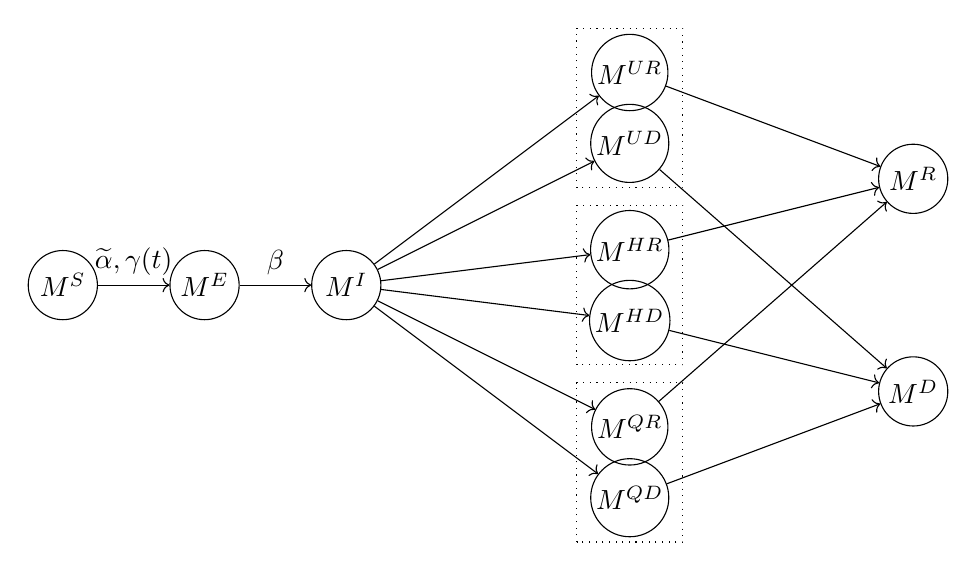
\begin{tikzpicture}[scale=0.45]
    \node[circ,draw=black] (S) at (0, 0){$M^S$};
    \node[circ,draw=black] (E) at (4,0){$M^E$};
    \node[circ,draw=black] (I) at (8,0) {$M^I$};
    
    \node[circ,draw=black] (UR) at (16,6) {$M^{UR}$};
    \node[circ,draw=black] (UD) at (16,4) {$M^{UD}$};
    \draw[dotted] (14.5,2.75) rectangle (17.5,7.25);

    \node[circ,draw=black] (HR) at (16,1) {$M^{HR}$};
    \node[circ,draw=black] (HD) at (16,-1) {$M^{HD}$};
    \draw[dotted] (14.5,-2.25) rectangle (17.5,2.25);

    \node[circ,draw=black] (QR) at (16,-4) {$M^{QR}$};
    \node[circ,draw=black] (QD) at (16,-6) {$M^{QD}$};
    \draw[dotted] (14.5,-7.25) rectangle (17.5,-2.75);

    \node[circ,draw=black] (R) at (24,3) {$M^R$};
    \node[circ,draw=black] (D) at (24,-3) {$M^D$};

    \draw[->] (S) -- (E) node[midway,above]{$\widetilde{\alpha}, \gamma(t)$};
    \draw[->] (E) -- (I) node[midway,above]{$\beta$};
    \draw[->] (I) -- (HR);
    \draw[->] (I) -- (HD);
    \draw[->] (I) -- (QR);
    \draw[->] (I) -- (QD);
    \draw[->] (I) -- (UD);
    \draw[->] (I) -- (UR);

    \draw[->] (QR) -- (R);
    \draw[->] (UR) -- (R);
    \draw[->] (HR) -- (R);
    \draw[->] (UD) -- (D);
    \draw[->] (HD) -- (D);
    \draw[->] (QD) -- (D);
\end{tikzpicture}
}
\caption{Flow Diagram of DELPHI.}
\label{fig:DELPHI}
\end{figure}
Figure~\ref{fig:DELPHI} depicts a flow representation of the model, where each arrow represents how individuals can flow between different states.
The underlying differential equations are governed by 16 parameters which are shown on the appropriate arrows in Figure~\ref{fig:DELPHI} and defined below. To limit the amount of data needed to train this model, only the parameters denoted with a tilde are being fitted against historical data for each area (country/state/province); the others are largely biological parameters that are fixed using available clinical data from a meta-analysis of over 190 papers on COVID-19 available at time of model creation \citepmain{bertsimas2020covidClinicalOutcomes}. A small selection of references for each parameter is given below.
\begin{itemize}[topsep=0pt,itemsep=0pt]
    \item $\widetilde{\alpha}$ is the baseline infection rate. 

    \item $\gamma(t)$ measures the effect of government response and is defined as:
    \[\gamma(t)=1 + \frac{2}{\pi}\arctan\left(\frac{-(t-\widetilde{t_0})}{\widetilde{k}}\right) + \widetilde{c}\exp\left(-\frac{(t-\widetilde{t_\text{jump}})^2}{2\widetilde{\sigma}^2}\right), \]
    where the parameters $\widetilde{t_0}$ and $\widetilde{k}$ capture, respectively, the timing and the strength of the response. The exponential term intends to reflect a resurgence in infections due to relaxation of governmental policy and societal response, where $\widetilde{c}$ controls the magnitude of resurgence, $\widetilde{t_\text{jump}}$ the time of the acme of the resurgence, and $\widetilde{\sigma}$ the duration of the resurgence phase.  The effective infection rate in the model is $\widetilde{\alpha}\gamma(t)$, which is time dependent. The $\frac{2}{\pi}$ constant is so that the starting $\gamma(t)$ with $\widetilde{c}=0$ is normalized to the range of $[0,2]$ with $\gamma(t)=1$ if $t=t_0$. This allows both $\gamma(t)$ and $\alpha$ to be identified and be used within the THEMIS model. 
    \item $r_d$ is the rate of detection. This equals to $\frac{\log 2}{T_{d}}$, where $T_{d}$ is the median time to detection (fixed to be 2 days), see  \citemain{wang2020evolving}.
    \item $\beta$ is the rate of infection leaving incubation phase. This equals to $\frac{\log 2}{T_{\beta}}$, where $T_{\beta}$ is the median time to leave incubation (fixed at 5 days), see  \citemain{lauer2020incubation}.
    \item $\sigma$ is the rate of recovery of non-hospitalized patients. This equals to $\frac{\log 2}{T_{\sigma}}$, where $T_{\sigma}$ is the median time to recovery of non-hospitalized patients  (fixed at 10 days), see \citemain{hu2020clinical,kluytmans2020sars}.
    \item $\kappa$ is the rate of recovery under hospitalization.  This equals to $\frac{\log 2}{T_{\kappa}}$, where $T_{\kappa}$ is the median time to recovery under hospitalization (fixed at 15 days), see \citemain{liu2020clinical,grein2020compassionate}.
    \item $\widetilde{\tau}$ is the rate of death. This captures the speed at which a dying patient dies, and thus inversely proportional to how long a dying patient stays alive.

    \item $\widetilde{\mu}(t)$ is the case fatality rate, defined as:
    \begin{align*}
        \widetilde{\mu}(t) = \left(\widetilde{\mu_0} - \mu_{\min}\right)\left(1 + \frac{2}{\pi}\arctan\left(-\widetilde{r_m} t\right)\right) + \mu_{\min},
\end{align*}
Where $\widetilde{\mu_0}$ is the initial case fatality rate, $\mu_{\min}$ is the minimum case fatality rate and $\widetilde{r_m}$ is the decay rate for mortality. This parametric curve describes the natural decay of case fatality rate as standard of care improves throughout the pandemic. Notice that this quantity measures the percentage of people who die from the disease in a particular region, and is independent from the rate of death. If $r_m<0$, this function can also capture the effect of an increasing mortality rate. 
    \item $p_d$ is the percentage of infectious cases detected, which is fixed at $20\%$ based on various reports trying to understand the extent of underdetection in countries with earlier outbreaks. \citemain{wang2020evolving, krantz2020level,niehus2020quantifying}
    \item $p_h$ is the (constant) percentage of detected cases hospitalized, which is set to $15\%$, see \citemain{arons2020presymptomatic,xu2020evaluation}.
\end{itemize}

We fit on 9 parameters from the list above ($\widetilde{\alpha}$,  $\widetilde{t_0}$, $\widetilde{k}$, 
 $\widetilde{c}$, $\widetilde{t_\text{jump}}$, $\widetilde{\sigma}$, $\widetilde{\mu_0}$, $\widetilde{r_m}, \$\widetilde{\tau}$). In addition, we introduce 2 additional parameters $\widetilde{k_1}$, $\widetilde{k_2}$ to account for the unknown initial population in the infected ($M^I$) and exposed ($M^E$) states. We thus fit 11 parameters per area.

The parameters are fitted by minimizing a weighted Mean Squared Error (MSE) metric with respect to the parameters. In general, other loss functions may be used as the calibration errors for a pandemic evolution are not necessarily random - however we have experimentally found that the MSE metric, which gives more prominence to days with larger number of cases and deaths, produce predictions that generalize better into the future.  Let  $M^{DT}(t)$ and $M^{DD}(t)$ denote  the number of reported total detected cases and detected deaths, respectively, on day $t$. Then, the loss function for a training period of $T$ days is defined as:
$$
\begin{aligned}
\sum_{t=1}^{T} \frac{t^2}{T^2} \cdot \left(\widetilde{M^{DT}}(t) - M^{DT}(t)\right)^2 + \lambda^2 \cdot \sum_{t=1}^{T} t \cdot \left(\widetilde{M^{DD}}(t) - M^{DD}(t)\right)^2,
\end{aligned}
$$
where $\widetilde{M^{DT}}(t)$ and $\widetilde{M^{DD}}(t)$ are respectively the total detected cases and deaths predicted by DELPHI. We utilize mean-squared error (MSE) for model calibration because it emphasizes larger errors, which is crucial for our application. Specifically, in the context of THEMIS, periods with a high number of cases contribute disproportionately to the overall cost. By using MSE, the calibration process prioritizes accuracy during these critical periods, ensuring that the model is more sensitive to situations where errors could have a significant impact. The factor $\frac{t^2}{T^2}$ gives more prominence to more recent data, as recent errors are more likely to propagate into future errors. The lambda factor $\lambda= \min\Big\{ \frac{M^{DT}(T)}{3\cdot M^{DD}(T)}, 10\Big\}$ balances the fitting between detected cases and deaths while the factor 10 avoids data stability issues due to low amount of deaths; this re-scaling coefficient was obtained experimentally through cross-validation on early pandemic data. We specifically exclude historical data starting before the area recorded more than 100 cases; this allows us to exclude sporadic outbreaks that are not epidemics. To optimize over the highly non-convex search space, we utilize both the local truncated newton algorithm (TNC) \citepmain{nocedal2006numerical} and the global optimization method of dual annealing (DA) \citepmain{xiang1997generalized}.TNC is utilized to produce forecasts on a daily basis while DA, being more computationally expensive, is performed on a weekly basis to shift and re-adjust the parameters more significantly if the underlying mechanics have changed (e.g. in the case of a new wave of cases). We use a bound of $20\%$ deviation around the latest value for TNC, and a bound of $50\%$ deviation for DA. 
\vfill
\newpage
\newpage
\section{List of Region-specific Cost Parameters}
\label{app:region_specific_params}

\subsection{Summary Table}
\begin{table}[H]
\centering
\resizebox{\textwidth}{!}{
\begin{tabular}{|l|c|c|c|c|}
\hline 
\textbf{Parameters} & \textbf{Germany} & \textbf{Spain} & \textbf{New York, US} & \textbf{Brazil} \\\hline
\textit{Cost of loss of life $c_{R,LL}$} &&&&\\
\hspace{2pt} COVID-19 deaths $l_R(u)$ &\citeapp{robert2021robert}&\citeapp{INED}&\citeapp{NYDoH}&\citeapp{BRDeaths}\\
\hspace{2pt} Actuarial tables $f_R(u)$ &\citeapp{SB-mortality}&\citeapp{INE-Mortality}&\citeapp{SSA}&\citeapp{IBGE-Mortality}\\
\hspace{2pt} Value of statistical life year $c_{R,VSLY}$ & \makecell{158,448 \\ \citepapp{schlander2017empirical}} & \makecell{158,448 \\ \citepapp{schlander2017empirical}}&\makecell{455,484 \\ \citepapp{robinson2021benefits}}&\makecell{247,803 \\ \citepapp{mardones2018estimation}}\\
\hspace{2pt} Age Upper Bound $U$ & \makecell{100\\ } & \makecell{100 \\ }&\makecell{100 \\ }& \makecell{100 \\ }\\
\hspace{2pt} Probability of Long-COVID $p_{LC}$ & \makecell{$6.6\%$\\ \citeapp{hastie2023true}} & \makecell{$6.6\%$\\ \citeapp{hastie2023true}}&\makecell{$6.6\%$\\ \citeapp{hastie2023true}}& \makecell{$6.6\%$\\ \citeapp{hastie2023true}}\\
\hspace{2pt} Time of Long COVID $T_{LC}$ & \makecell{5 Years\\ \citeapp{davis2021characterizing}} & \makecell{5 Years\\ \citeapp{davis2021characterizing}}&\makecell{5 Years\\ \citeapp{davis2021characterizing}}& \makecell{5 Years\\ \citeapp{davis2021characterizing}}\\
\hspace{2pt} Loss in Utility $\Delta l$ & \makecell{$10\%$\\ \citeapp{martin2021model}} & \makecell{$10\%$\\ \citeapp{martin2021model}}&\makecell{$10\%$\\ \citeapp{martin2021model}}& \makecell{$10\%$\\ \citeapp{martin2021model}}\\
\hline
\textit{Hospitalization Cost $c_{R,H}$} &&&&\\
\hspace{2pt} Inpatient $c^D_{R,H}$ &\makecell{162 \\ \citepapp{kaier2020mechanical}}&\makecell{353 \\ \citepapp{iFHP}}&\makecell{2,250 \\ \citepapp{BCBS2021}}&\makecell{593 \\ \citepapp{santos2021public}}\\
\hspace{2pt} ICU $c^D_{R,I}$&\makecell{795 \\ \citepapp{kaier2020mechanical}} &\makecell{1,700 \\ \citepapp{bittner2013intensive}} &\makecell{5,625 \\ \citepapp{BCBS2021}}&\\
\hspace{2pt} ICU+Ventilation $c^D_{R,V}$ & \makecell{1539 \\\citepapp{kaier2020mechanical}}& \makecell{2,703 \\ \citepapp{bittner2013intensive}}&\makecell{7,010 \\ \citepapp{BCBS2021}}&\\\hline
\textit{Economic Cost $c_{R,Y}$} &&&&\\
\hspace{2pt} GDP $C_R, I_R, G_R, NX_R$&\makecell{$3.86 \times 10^{12}$ \\ \citepapp{IMF20}}&\makecell{$1.25 \times 10^{12}$ \\ \citepapp{IMF20}}&\makecell{$1.77 \times 10^{12}$ \\ \citepapp{BEA20}}&\makecell{$1.25 \times 10^{12}$ \\ \citepapp{IMF20}}\\ 
\hspace{2pt} Total number of working days $T_{R,W}$ &\makecell{$254$ \\ \citepapp{IMF20}}&\makecell{$252$ \\ \citepapp{IMF20}}&\makecell{$261$ \\ \citepapp{BEA20}}& \makecell{252 \\ \citepapp{IMF20}}\\
\hspace{2pt} Average days of sickness $T_S$ &\makecell{$10$ \\ \citepapp{cascini2022cross}}&\makecell{$10$ \\ \citepapp{cascini2022cross}}&\makecell{$10$ \\ \citepapp{cascini2022cross}}& \makecell{$10$ \\ \citepapp{cascini2022cross}}\\
\hline
\textit{Mental Health Cost $c_{R,M}$} &&&&\\
\hspace{2pt} Cost of MDD $c_{R,Dep}$ &\makecell{3,813 \\ \citepapp{rybakowski2014mddcost}}&\makecell{3,412 \\ \citepapp{vieta2021esmddcost}}&\makecell{37,932 \\ \citepapp{greenberg2015economic}}&\makecell{4,100 \\ \citepapp{lepine2012mddcost}}\\
\hspace{2pt} Cost of PTSD $c_{R,PTSD}$ &\makecell{8,600 \\ \citepapp{bothe2020ptsdcost}}&\makecell{8,600 \\ \citepapp{bothe2020ptsdcost}}&\makecell{14,857 \\ \citepapp{bothe2020expensive}}&\makecell{4,100 \\ \citepapp{lepine2012mddcost}}\\
\hspace{2pt} No. of Healthcare Workers $N_{R,H}$ &\makecell{892,000 \\ \citepapp{destatisHealthcareWorkersDE}}&\makecell{542,140 \\ \citepapp{msssi_2019}}&\makecell{600,000 \\ \citepapp{nyhcw}}&\makecell{2,579,430 \\ \citepapp{wbbr20}}\\
\hspace{2pt} General Population over 14 $N_R$ &\makecell{72,520,000 \\ \citepapp{wbdepop20}}&\makecell{39,756,493 \\ \citepapp{wbespop20}}&\makecell{16,164,571 \\ \citepapp{nydohpop}}&\makecell{43,695,990 \\ \citepapp{wbbrpop20}}\\
\hspace{2pt} Baseline Depression rate &\makecell{7.6\% \\ \citepapp{dedepression}}&\makecell{4.7\%  \\ \citepapp{vieta2021esmddcost}}&\makecell{8.5\%  \\ \citepapp{ettman2020depression}}&\makecell{3.9\%  \\\ \citepapp{FETER2021101depression}}\\
\hspace{2pt} Depression rate increase $\Delta r_{R,Dep}$&\makecell{6.7\% \\ \citepapp{dedepression}}&\makecell{14.0\% \\ \citepapp{sanguino2020es}}&\makecell{19.3\% \\ \citepapp{ettman2020depression}}&\makecell{25.2\% \\ \citepapp{FETER2021101depression}}\\
\hspace{2pt} Baseline PTSD rate &\makecell{2.3\%  \\ \citepapp{deptsdbaseline}}&\makecell{0.57\%  \\ \citepapp{wittchen2011size}}&\makecell{3.6\%  \\ \citepapp{nimhusptsd}}&\makecell{4.3\%  \\ \citepapp{dasilva2019ptsd}}\\
\hspace{2pt} PTSD rate increase $\Delta r_{R,PTSD}$&\multirow{ 2}{*}{\makecell{27.7\% \\ \citepapp{georgieva2021prevalence}}}&\multirow{ 2}{*}{\makecell{15.2\% \\ \citepapp{sanguino2020es}}}&\multirow{ 2}{*}{\makecell{30.7\% \\ \citepapp{liu2020factorsapp,bryant2021symptoms}}}&\multirow{ 2}{*}{\makecell{30.0\% \\ \citepapp{GOULARTE202132}}}\\
\\\hline
\textit{Unemployment Cost $c_{R,U}$} &&&&\\
\hspace{2pt} Total Labor Force $N_{R,W}$&\makecell{43,356,000 \\ \citepapp{wbde20}} &\makecell{22,694,625 \\ \citepapp{wbes20}} &\makecell{9,500,000 \\ \citepapp{bls20}}&\makecell{107,461,083 \\ \citepapp{wbbr20}}\\
\hspace{2pt} Unemployment $U_R(i)$ & \citeapp{SB-unemployment} & \citeapp{oecd_2024} & \citeapp{nyunemployment} & \citeapp{IBGE-Unemployment}\\
\hspace{2pt} Unemployment Cost $c^Y_{R,U}$ & \makecell{77,510 \\\citepapp{chen2019effect}}& \makecell{66,312 \\ \citepapp{gorjon2018social}}&\makecell{60,000 \\ \citepapp{blanchflower2004well}}&\makecell{52,557 \\ \citepapp{chen2019effect}}\\\hline

\end{tabular}
}
\caption{Values and sources for the THEMIS parameters used in Section \ref{sec:experiment}. All monetary units are in local currency units unless otherwise specified. The values referenced here correspond to the year of measurement. For sources with monetary information not from the simulation year (2020), we correct the monetary value using the Consumer Price Index for that region.}
\end{table}
\subsection{Detailed Justification}
\subsubsection{General Strategy}
For all sources, our objective is to identify the most recent peer-reviewed references relevant to the subject population. Population relevance is given higher priority than recency. This means that, for data specific to Spain, a study analyzing Spanish data from 2004 would be prioritized over a study analyzing pan-European data from 2020. If no data specific to the target region is available, we will seek the most relevant source following a hierarchical approach: first, by considering the superset region (e.g., for Spain, this would be Europe; for New York, it would be the United States). If no relevant data is available at this level, we will then look for the best available source from another country within the same super-region. This reference strategy is visually summarized in the flow diagram below:
\begin{figure}[htbp!]
\centering
\tikzstyle{process} = [rectangle, minimum width=3cm, minimum height=1cm, text centered, draw=black, fill=orange!30]
\resizebox{0.75\textwidth}{!}{
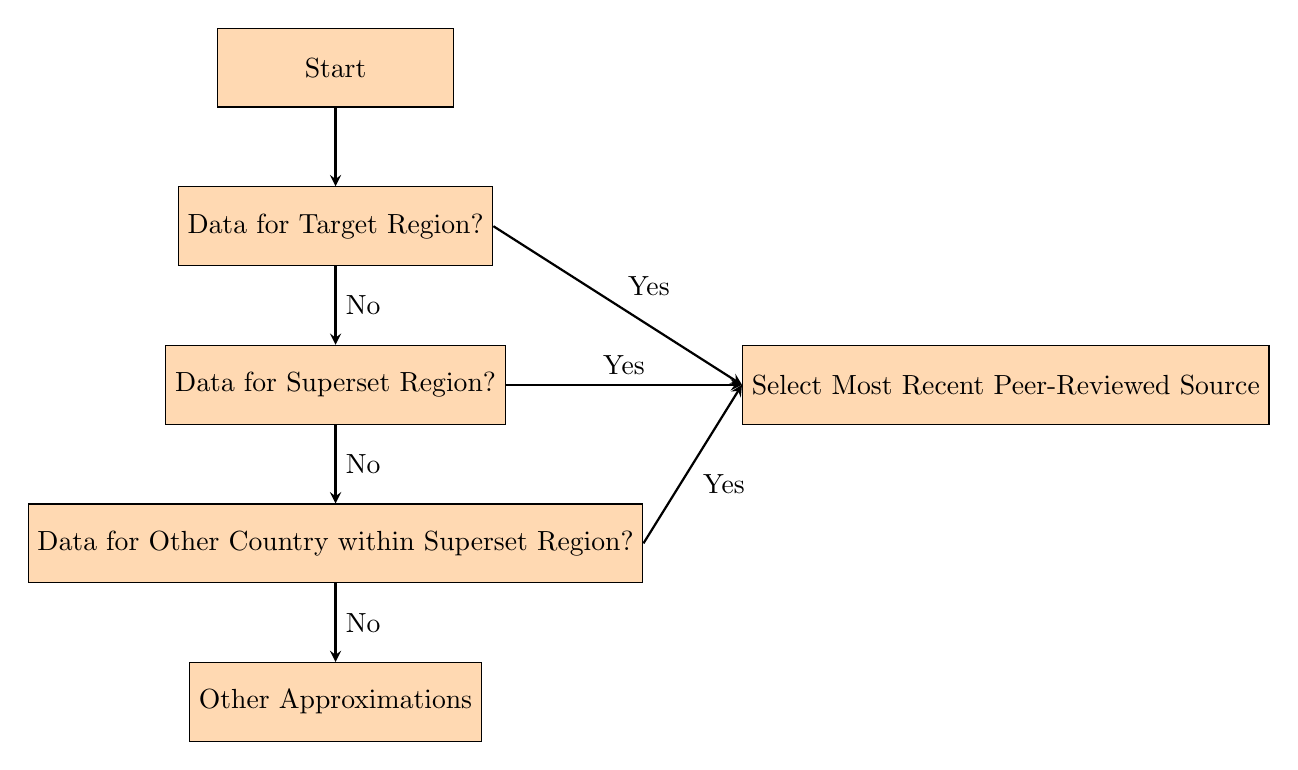
\begin{tikzpicture}[
    node distance=1cm and 1.5cm,
    every edge/.style={draw, thick, -{Latex[length=3mm, width=2mm]}}
    ]

    % Nodes
    \node (start) [process] {Start};
    \node (target) [process, below=of start] {Data for Target Region?};
    \node (superset) [process, below=of target] {Data for Superset Region?};
    \node (other) [process, below=of superset] {Data for Other Country within Superset Region?};
    \node (recent) [process, right=3cm of superset] {Select Most Recent Peer-Reviewed Source};
    \node (best) [process, below=of other] {Other Approximations};

    % Edges
    \draw[arrow] (start) -- (target);
    \draw[arrow] (target) -- node [pos=0.5, right] {No} (superset);
    \draw[arrow] (superset) -- node [pos=0.5, right] {No} (other);
    \draw[arrow] (other) -- node [pos=0.5, right] {No} (best);
    \draw[arrow] (target.east) -- node [pos=0.5, above right] {Yes} (recent.west);
    \draw[arrow] (superset.east) -- node [pos=0.5, above] {Yes} (recent.west);
    \draw[arrow] (other.east) -- node [pos=0.5, below right] {Yes} (recent.west);
\end{tikzpicture}
}
\caption{Flow Diagram for Source Validation}
\end{figure}

If there are multiple sources that each pertain to a subset of the target population (e.g. for the increase in depression prevalence in United States, there are two sources on the increase in depression prevalence for doctors and young adults), their results are averaged to give the final estimate.

\subsubsection{Globally Fixed Parameters}

\paragraph{Age Upper Bound ($U$):} The age upper bound is uniformly set at 100 years across all regions in this study. For the four regions considered, the percentage of the population aged 100 and above is presented in Table \ref{tab:age100}, with values all below $0.03\%$. Given that centenarians are typically expected to live only 1-2 additional years without COVID-19 \citepapp{sebastiani2012,centenarian_stats}, their contribution to the total cost of deaths, $c_{R,D}$, is estimated to be less than $0.03\%$, which is negligible compared to the overall model uncertainty.

\begin{table}[h!]
\centering
\caption{\label{tab:age100} Percentage of Population Aged 100 and Over in Selected Regions (2024)}
\begin{tabular}{cccc}
\toprule
\textbf{Germany} & \textbf{Spain} & \textbf{New York, US} & \textbf{Brazil} \\
\citepapp{germany2024} & \citepapp{spain2024} & \citepapp{pew2024} & \citepapp{brazil2024} \\
\midrule
0.031\% & 0.021\% & 0.03\% & 0.01\% \\
\bottomrule
\end{tabular}
\end{table}

\paragraph{Long COVID Parameters ($p_{LC}$, $T_{LC}$, and $\Delta l$):} Estimating the prevalence, duration, and impact of Long COVID is challenging due to ongoing uncertainties and the variety of possible symptoms. Prevalence estimates often rely on survey data, which may be confounded by biases such as self-reporting. For this study, we adopt the prevalence rate from the largest population cohort available at the time \citepapp{hastie2023true}, assuming it to be globally applicable. Duration and impact estimates follow the strategy in \citeapp{cutler2022economic}, assuming Long COVID persists for an average of 5 years with a $10\%$ reduction in quality of life during this period \citepapp{davis2021characterizing,martin2021model}.
\paragraph{Average Days of Sickness ($T_S$):} The recovery period for mild to moderate COVID-19 cases typically averages around two weeks, with minimal variation across countries \citepapp{cascini2022cross,tenforde2020symptom}. We assume 10 of these days are working days, thus setting $T_S = 10$.

\subsubsection{Germany}
\paragraph{COVID-19 Deaths ($I_R(u)$):} Data is sourced from the Robert Koch Institute.
\paragraph{Actuarial Tables ($f_R(u)$):} The latest pre-COVID actuarial tables (2018/2020) are utilized from the German Federal Statistical Office (Destatis).
\paragraph{Value of Statistical Life Year ($c_{R,VSLY}$):} The most recent estimate for the value of a statistical life year is taken from \citeapp{schlander2017empirical}, calculated in 2017.

\paragraph{Hospitalization Costs ($c^D_{R,H}$, $c^D_{R,I}$, $c^D_{R,V}$):} ICU and ventilated patient cost estimates are based on the respiratory subgroup (Subgroup X) from \citeapp{kaier2020mechanical}. For general hospitalization costs, we take data from the German Federal Statistical Office stating inpatient cost is roughly $1/5$th as expensive as ICU. 
\paragraph{GDP ($C_R, I_R, G_R, NX_R$):} Relevant GDP data is obtained from the IMF database \citepapp{IMF20}, which categorizes GDP components as defined.
\paragraph{Total Number of Working Days ($T_{R,W}$):} Data on working days is also sourced from the IMF database.
\paragraph{Cost of Major Depressive Disorder (MDD) ($c_{Dep}$):} The most recent annual estimates for depression-related costs are derived from \citeapp{rybakowski2014mddcost}.
\paragraph{Cost of PTSD ($c_{PTSD}$):} The total cost for PTSD over a 5-year period is reported as \euro43,000 by \citeapp{bothe2020expensive}, which we approximate to \euro8,600 annually.
\paragraph{Number of Healthcare Workers ($N_{R,H}$):} Data is sourced from the German Federal Statistical Office.
\paragraph{General Population over 14 ($N_{R}$):} Population data is taken from 2020 World Bank statistics.
\paragraph{Depression Rate Increase ($\Delta r_{Dep}$):} A cross-sectional study by \citeapp{dedepression} during Germany’s severe lockdown measures found that the prevalence of major depression (defined by PHQ-2 sum scores $\geq 3$) increased from 7.6\% to 14.3\%, reflecting a 6.7\% increase.

\paragraph{PTSD Rate Increase ($\Delta r_{PTSD}$):} \citeapp{deptsdbaseline} reports a baseline PTSD prevalence of $2.3\%$ in Germany. Due to the lack of specific data on PTSD prevalence in Germany during the COVID-19 pandemic, we applied an average from a survey conducted across 10 European countries (excluding India), which found a pandemic-era prevalence of $30.0\%$ \citepapp{georgieva2021prevalence}. This suggests a significant increase of $27.7\%$ in PTSD prevalence during the pandemic.

\paragraph{Total Labor Force ($N_{R,W}$):} Data is sourced from the 2020 World Bank database.

\paragraph{Unemployment ($U_R(i)$):} Unemployment figures are obtained from the German Federal Statistical Office.

\paragraph{Unemployment Cost ($c^Y_{R,U}$):} An analysis by \citeapp{chen2019effect} indicates that in Germany, the impact of unemployment is $\approx22\%$ greater than a drop from the top income quintile to the lowest. This is then converted to anumber using income data from OECD database \citepapp{oecd2024idd}.


\subsubsection{Spain}
\paragraph{COVID-19 Deaths ($I_R(u)$):} Data is collected from the \emph{Institut national d'études démographiques}, which aggregates data from Spain’s Ministry of Health, Consumption, and Social Welfare (MSCBS).
\paragraph{Actuarial Tables ($f_R(u)$):} The latest pre-COVID actuarial tables (2019) are sourced from the Spanish National Statistics Institute.
\paragraph{Value of Statistical Life Year ($c_{R,VSLY}$):} The most recent estimate for the value of a statistical life year is obtained from \citeapp{schlander2017empirical}, calculated in 2017.
\paragraph{Hospitalization Costs ($c^D_{R,H}$, $c^D_{R,I}$, $c^D_{R,V}$):} General inpatient costs come from the International Federation of Health Plans \cite{iFHP}, with ICU and ventilated patient costs  from Table 2 in \citeapp{bittner2013intensive}.
\paragraph{GDP ($C_R, I_R, G_R, NX_R$):} GDP components are sourced from the IMF database \citepapp{IMF20}.

\paragraph{Total Number of Working Days ($T_{R,W}$):} This is obtained from the IMF database \citepapp{IMF20}.
\paragraph{Cost of Major Depressive Disorder (MDD) ($c_{Dep}$):} Recent cost estimates for treating depression in Spain (2015-2017) are based on an observational study by \citeapp{vieta2021esmddcost}.
\paragraph{Cost of PTSD ($c_{PTSD}$):} In the absence of Spain-specific data, we use the German estimate from \citeapp{bothe2020expensive}, assuming an annual cost of \euro8,600.
\paragraph{Number of Healthcare Workers ($N_{R,H}$):} Data is sourced from Spain’s Ministry of Health, Social Services, and Equality.
\paragraph{General Population over 14 ($N_{R}$):} Population data is sourced from the 2020 World Bank database.
\paragraph{Depression Rate Increase ($\Delta r_{Dep}$):} \citeapp{vieta2021esmddcost}'s observational analysis from 2015-2017 revealed that the prepandemic prevalence of depressive disorders was $4.7\%$. In an online survey conducted during the initial stages of the pandemic, \citepapp{sanguino2020es} found $18.7\%$ of the sample had symptomatic depression (on the PHQ-2 scale), representing a $14.0\%$ increase from the baseline. 


\paragraph{PTSD Rate Increase $\Delta r_{PTSD}$:} The baseline PTSD depression rate comes from a 2010 Europe-wide study \citeapp{wittchen2011size} that indicated Spain had a low prevalence ($0.57\%$) of PTSD. In the same online survey as the depression data, \citepapp{sanguino2020es} found $15.8\%$ of the sample had symptomatic PTSD, representing a $15.2\%$ increase from the baseline. 
\paragraph{Total Labor Force ($N_{R,W}$):} Data is sourced from the 2020 World Bank database.

\paragraph{Unemployment ($U_R(i)$):} Unemployment data is published by the OECD and accessed via the FRED system \citepapp{oecd_2024}.

\paragraph{Unemployment Cost ($c^Y_{R,U}$):} An analysis by \citeapp{gorjon2018social} on Spain’s social cost of unemployment estimates a monthly cost of \euro5,526, translating to an annual cost of \euro66,312.

\subsubsection{New York, US}

\paragraph{COVID-19 Deaths ($I_R(u)$):} Data is taken from the New York Department of Health. \citepapp{NYDoH}
\paragraph{Actuarial Tables ($f_R(u)$):} We utilize the latest pre-pandemic actuarial life table from the Social Security Administration in 2019. \citepapp{SSA}
\paragraph{Value of Statistical Life Year ($c_{R,VSLY}$):} \citeapp{robinson2021benefits} provides the latest available estimate of VSLY in the United States. We take the constant VSLY estimate from the paper that is corrected with the $3\%$ discount rate.
\paragraph{Hospitalization Costs ($c^D_{R,H}$, $c^D_{R,I}$, $c^D_{R,V}$):} \citeapp{BCBS2021} provides an estimate of the cost of COVID-19 hospitalization with and without an ICU stay. We calculate the daily cost by dividing the total by an average 15-day hospitalization period as estimated by \citeapp{li:20app}. For ICU and ventilated patient costs, we use the daily ICU cost without ventilation from \citeapp{dasta2005daily} ($\$3,184$ per day) and adjust for ventilation costs ($\$3,968$ per day) using the ratio $3968/3184$.


\paragraph{GDP ($C_R, I_R, G_R, NX_R$):} We take the relevant data from the Bureau of Economic Analysis that divides the GDP into the respective categories as defined. 
\paragraph{Total Number of Working Days ($T_{R,W}$):} This is obtained from \cite{BEA20}.

\paragraph{Cost of MDD ($c_{Dep}$):} We use latest cost estimates for depression in the US from \citeapp{greenberg2015economic}.


\paragraph{Cost of PTSD ($c_{PTSD}$):} \citeapp{davis2022economic} reports that yearly PTSD cost in the US was \$19,630 (2018).

\paragraph{Number of Healthcare Workers ($N_{R,H}$):} Data from Center for Disease Control and Prevention (CDC).

\paragraph{General Population over 14 ($N_{R}$):} Population data is sourced from the New York Department of Health \citepapp{nydohpop}.
\paragraph{Depression Rate Increase ($\Delta r_{Dep}$):} \citeapp{ettman2020depression} compared the prevalence of depression in the general US population before and after the pandemic. We included only those that exhibited moderate symptoms or above on the PHQ-9 scale (scoring 10 or above) to consistently correspond with the cutoff we utilize for the PHQ-2 scale for Germany. The pre-pandemic total prevalence was $8.5\%$ and the post-pandemic total prevalence was $27.8\%$, giving an increase of $19.3\%$. This increase appears to correspond well with other smaller surveys that focused on particular groups of individuals within the US \citepapp[e.g.][]{young2021hcwmentalhealth}. 

\paragraph{PTSD Rate Increase ($\Delta r_{PTSD}$):} Baseline PTSD estimates come from the National Institute of Mental Health \citeapp{nimhusptsd}. Pandemic-era prevalence data, though not available for the general population, shows consistent increases in specific groups, such as young adults \citepapp{liu2020factorsapp} and clinical staff \citepapp{bryant2021symptoms}, averaging a prevalence rate of 34.3\%, a 30.7\% increase from the baseline.

\paragraph{Total Labor Force ($N_{R,W}$):} This is sourced from the 2020 release by the Bureau of Labor Statistics.

\paragraph{Unemployment ($U_R(i)$):} Published by the FRED system at the St. Louis Federal Reserve Bank.

\paragraph{Unemployment Cost ($c^Y_{R,U}$):} \citeapp{blanchflower2004well} shows that unemployment creates a cost comparable to a \$60,000 income loss annually. This is consistent with \citeapp{chen2019effect}, estimating unemployment costs equivalent to 1.5 years of GDP per capita (approximately \$61,500 USD in 2019).




\subsubsection{Brazil}
\paragraph{COVID-19 Deaths ($I_R(u)$):} Data is collected from the COVID-19 dashboard maintained by the Fiocruz Foundation in Brazil, which offers the most detailed COVID-19 death data available at the time of writing.
\paragraph{Actuarial Tables ($f_R(u)$):} The latest pre-COVID actuarial tables are taken directly from the Brazilian Institute of Geography and Statistics.
\paragraph{Value of Statistical Life Year ($c_{R,VSLY}$):} \citeapp{mardones2018estimation} provides the latest estimate of the value of a statistical life (VSL) at \$1.19 million USD. We convert VSL to VSLY using the standard formula by \citeapp{moore1988quantity} with a 3\% discount rate (to be consistent with the USA estimate above) and life expectancy data from the Brazilian Institute of Geography and Statistics.
\paragraph{Hospitalization Costs ($c^D_{R,H}$, $c^D_{R,I}$, $c^D_{R,V}$):} We were unable to locate distinct cost estimates for hospitalization across inpatient, ICU, and ventilated patients. The only available source, \citeapp{santos2021public}, provided a generalized cost estimate for COVID-19 hospitalizations. Thus, we relied on this blended cost.
\paragraph{GDP ($C_R, I_R, G_R, NX_R$):} We take the relevant data from the IMF database \citepapp{IMF20} that divides the GDP into the respective categories as defined. 
\paragraph{Total Number of Working Days ($T_{R,W}$):} We take the relevant data from the IMF database.

\paragraph{Cost of MDD and PTSD ($c_{Dep}, c_{PTSD}$):} \citeapp{lepine2012mddcost} reports that the annual cost for typical MDD patients (without treatment-resistant depression) in Brazil is \$3,042 reals. We were unable to find references for the cost of treating PTSD patients in either Brazil or more generally for South America. For PTSD, given the lack of specific data, we assume the cost is comparable to that of MDD. Sensitivity analysis shows that even a fivefold increase in PTSD costs does not significantly impact our conclusions.

\paragraph{Number of Healthcare Workers ($N_{R,H}$):} Data is sourced from the 2020 statistics by the World Bank.

\paragraph{General Population over 14 ($N_{R}$):} Data is sourced from the 2020 statistics by the World Bank.
\paragraph{Depression Rate Increase ($\Delta r_{Dep}$):} \citeapp{FETER2021101depression} conducted a retrospective cohort study to measure the depression prevalence before/after  the start of the COVID-19 pandemic. The results show pre-pandemic prevalence of moderate or severe depression was $3.9\%$ and post-pandemic prevalence was $29.1\%$. 

\paragraph{PTSD Rate Increase ($\Delta r_{PTSD}$):} Pre-pandemic PTSD prevalence data comes from \citeapp{dasilva2019ptsd}, indicating a 4.2\% baseline. A web-based survey during the early pandemic months reported a PTSD prevalence of 34.2\%, a 30.0\% increase. \citepapp{GOULARTE202132}

\paragraph{Total Labor Force ($N_{R,W}$):} Labor force data is sourced from the 2020 World Bank statistics.

\paragraph{Unemployment ($U_R(i)$):} Unemployment data is directly sourced from the Brazilian Institute of Geography and Statistics.

\paragraph{Unemployment Cost ($c^Y_{R,U}$):} \citeapp{chen2019effect} suggests that unemployment costs are roughly equivalent to 1.5 years of GDP per capita. We extrapolate this using Brazil's 2019 GDP per capita.
\section{Regional Adjustment Factor and Error}
\label{app:adjustment_factor}
\begin{table}[h!]
\centering
\begin{tabular}{|l|c|c|}
\hline
\textbf{Country} & $k_R$ & $\sigma(k_R)$ \\ \hline
Brazil  & 1.043 & 0.020 \\ \hline
Germany & 0.286 & 0.084 \\ \hline
New York, US & 0.549 & 0.114 \\ \hline
Spain      & 0.442 & 0.019 \\ \hline
\end{tabular}
\caption{Table of $k_R$ and $\sigma(k_R)$ for different countries.}
\label{tab:kr_values}
\end{table}

\section{Empirical Validation of the Separability Assumption}
\label{app:separability}

A key assumption in Section \ref{subsec:delphi} is the separable structure $\gamma_{R,i} = k_R \gamma_i + \epsilon_R$, which implies that the matrix $\Gamma \in \mathbb{R}^{|R| \times |\mathcal{I}|}$ of region--policy effects is approximately rank-1. In this section, we provide rigorous empirical validation of this assumption across three distinct time periods of the pandemic.

\subsection*{Low-Rank Structure: Formulation}
We generalize the separability assumption by considering the matrix $\Gamma$ with entries $\gamma_{R,i}$ as a potentially low-rank matrix. Specifically, we consider the model:
\begin{equation}
    \Gamma \approx U V^\top, \qquad U \in \mathbb{R}^{|R| \times l},\; V \in \mathbb{R}^{|\mathcal{I}| \times l},
\end{equation}
where $l$ is the effective rank. The current model (Equation \ref{eq:uobsgamma}) corresponds to $l = 1$, with $U = \mb{k}$ (the vector of regional adjustment factors) and $V = \bm{\gamma}$ (the vector of global policy effects). Low-rank assumptions are commonly used for counterfactual analysis in observational data with multiple units. For example, \citeapp{athey2021matrix} uses a low-rank model for matrix completion of panel data, \citeapp{bai2009panel} develops panel data models with interactive fixed effects relying on a low-rank factor structure, and \citeapp{agarwal2021synthetic} proposes synthetic interventions using low-rank factor models.

To test whether $l = 1$ is adequate, we assemble the observed $\gamma_{R,i}$ values from 210 regions worldwide and 7 NPI categories across three time periods: 2020.03.15--2020.06.15, 2020.06.15--2020.09.15, and 2020.09.15--2020.12.15. Since $\gamma_{R,i}$ represents an infection-rate multiplier, we impose the physical constraint $\gamma_{R,i} \geq 0$. Both factors $K^{(l)}$ and $G^{(l)}$ are estimated from observed data via non-negative alternating least squares \citeapp{lee2001algorithms,xu2012alternating}. We use a \textbf{holdout RMSE} test: we randomly withhold 20\% of observed entries, estimate the rank-$l$ model on the remainder, and compute $\text{RMSE}_l = \sqrt{|\Omega_{\text{test}}|^{-1}\sum_{(R,i)\in\Omega_{\text{test}}} (\hat{\gamma}_{R,i}^{(l)} - \gamma_{R,i})^2}$, averaged over 20 random splits.

\subsection*{Multi-Period Holdout Analysis}

Table \ref{tab:svd_results} reports the holdout RMSE for rank-$l$ models ($l = 1, 2, 3$) across the three time periods.

\begin{table}[h!]
\centering
\begin{tabular}{|c|c|c|c|}
\hline $l$ & 2020.03.15--2020.06.15 & 2020.06.15--2020.09.15 & 2020.09.15--2020.12.15\\\hline
1 & $0.378 \pm 0.042$ & $0.287 \pm 0.026$ & $0.296 \pm 0.019$ \\
2 & $0.420 \pm 0.062$ & $0.292 \pm 0.030$ & $0.296 \pm 0.019$ \\
3 & $0.391 \pm 0.042$ & $0.289 \pm 0.025$ & $0.297 \pm 0.020$ \\\hline
\% observed & 24.9\% & 19.9\% & 20.0\% \\\hline
\end{tabular}
\caption{Holdout RMSE (mean $\pm$ std.\ over 20 random splits) for rank-$l$ non-negative models across three pandemic periods (20\% held out). Both factors $K^{(l)}$ and $G^{(l)}$ are estimated from data via non-negative alternating least squares. The rank-1 model achieves the lowest RMSE in Periods~1 and~2, and is tied in Period~3.}
\label{tab:svd_results}
\end{table}

The rank-1 model achieves the lowest holdout RMSE in two of three periods and is tied in the third. In Period~1, both rank-2 ($0.420 \pm 0.062$) and rank-3 ($0.391 \pm 0.042$) yield higher RMSE than rank-1 ($0.378 \pm 0.042$). In Periods~2 and~3, all ranks produce comparable RMSE within one standard deviation. Higher-rank models do not improve out-of-sample fit due to the extreme sparsity of the observation matrix (median 2 observed entries per region out of 7 policies), which leaves additional latent factors underdetermined.

\textbf{Remark on identifiability.} The rank-$l$ models for $l \geq 2$ are estimated via iterative truncated SVD with non-negative projection, warm-started from the converged rank-1 solution. With a median of 2 observed entries per region out of 7 policy categories (24.9\% observation rate in Period~1), higher-rank models are severely underdetermined---a rank-3 model requires 3 latent factors per region, but most regions have at most 2 observations to constrain them. The fact that neither rank-2 nor rank-3 improves upon rank-1 provides strong evidence that the rank-1 separability assumption captures all identifiable structure in the data: the region--policy interaction matrix is well-approximated by a single factor $k_R g_i$, and increasing model complexity does not improve predictive accuracy.

\subsection*{Rank-1 vs.\ Rank-2 and Rank-3 Comparison}

To further validate robustness, we compare the imputed $\gamma_{R,i}$ values from the rank-1 model against both rank-2 and rank-3 directly. Figure \ref{fig:rank1_vs_rank3_scatter_app} shows scatter plots for both comparisons across all three periods.

\begin{figure}[h!]
\centering
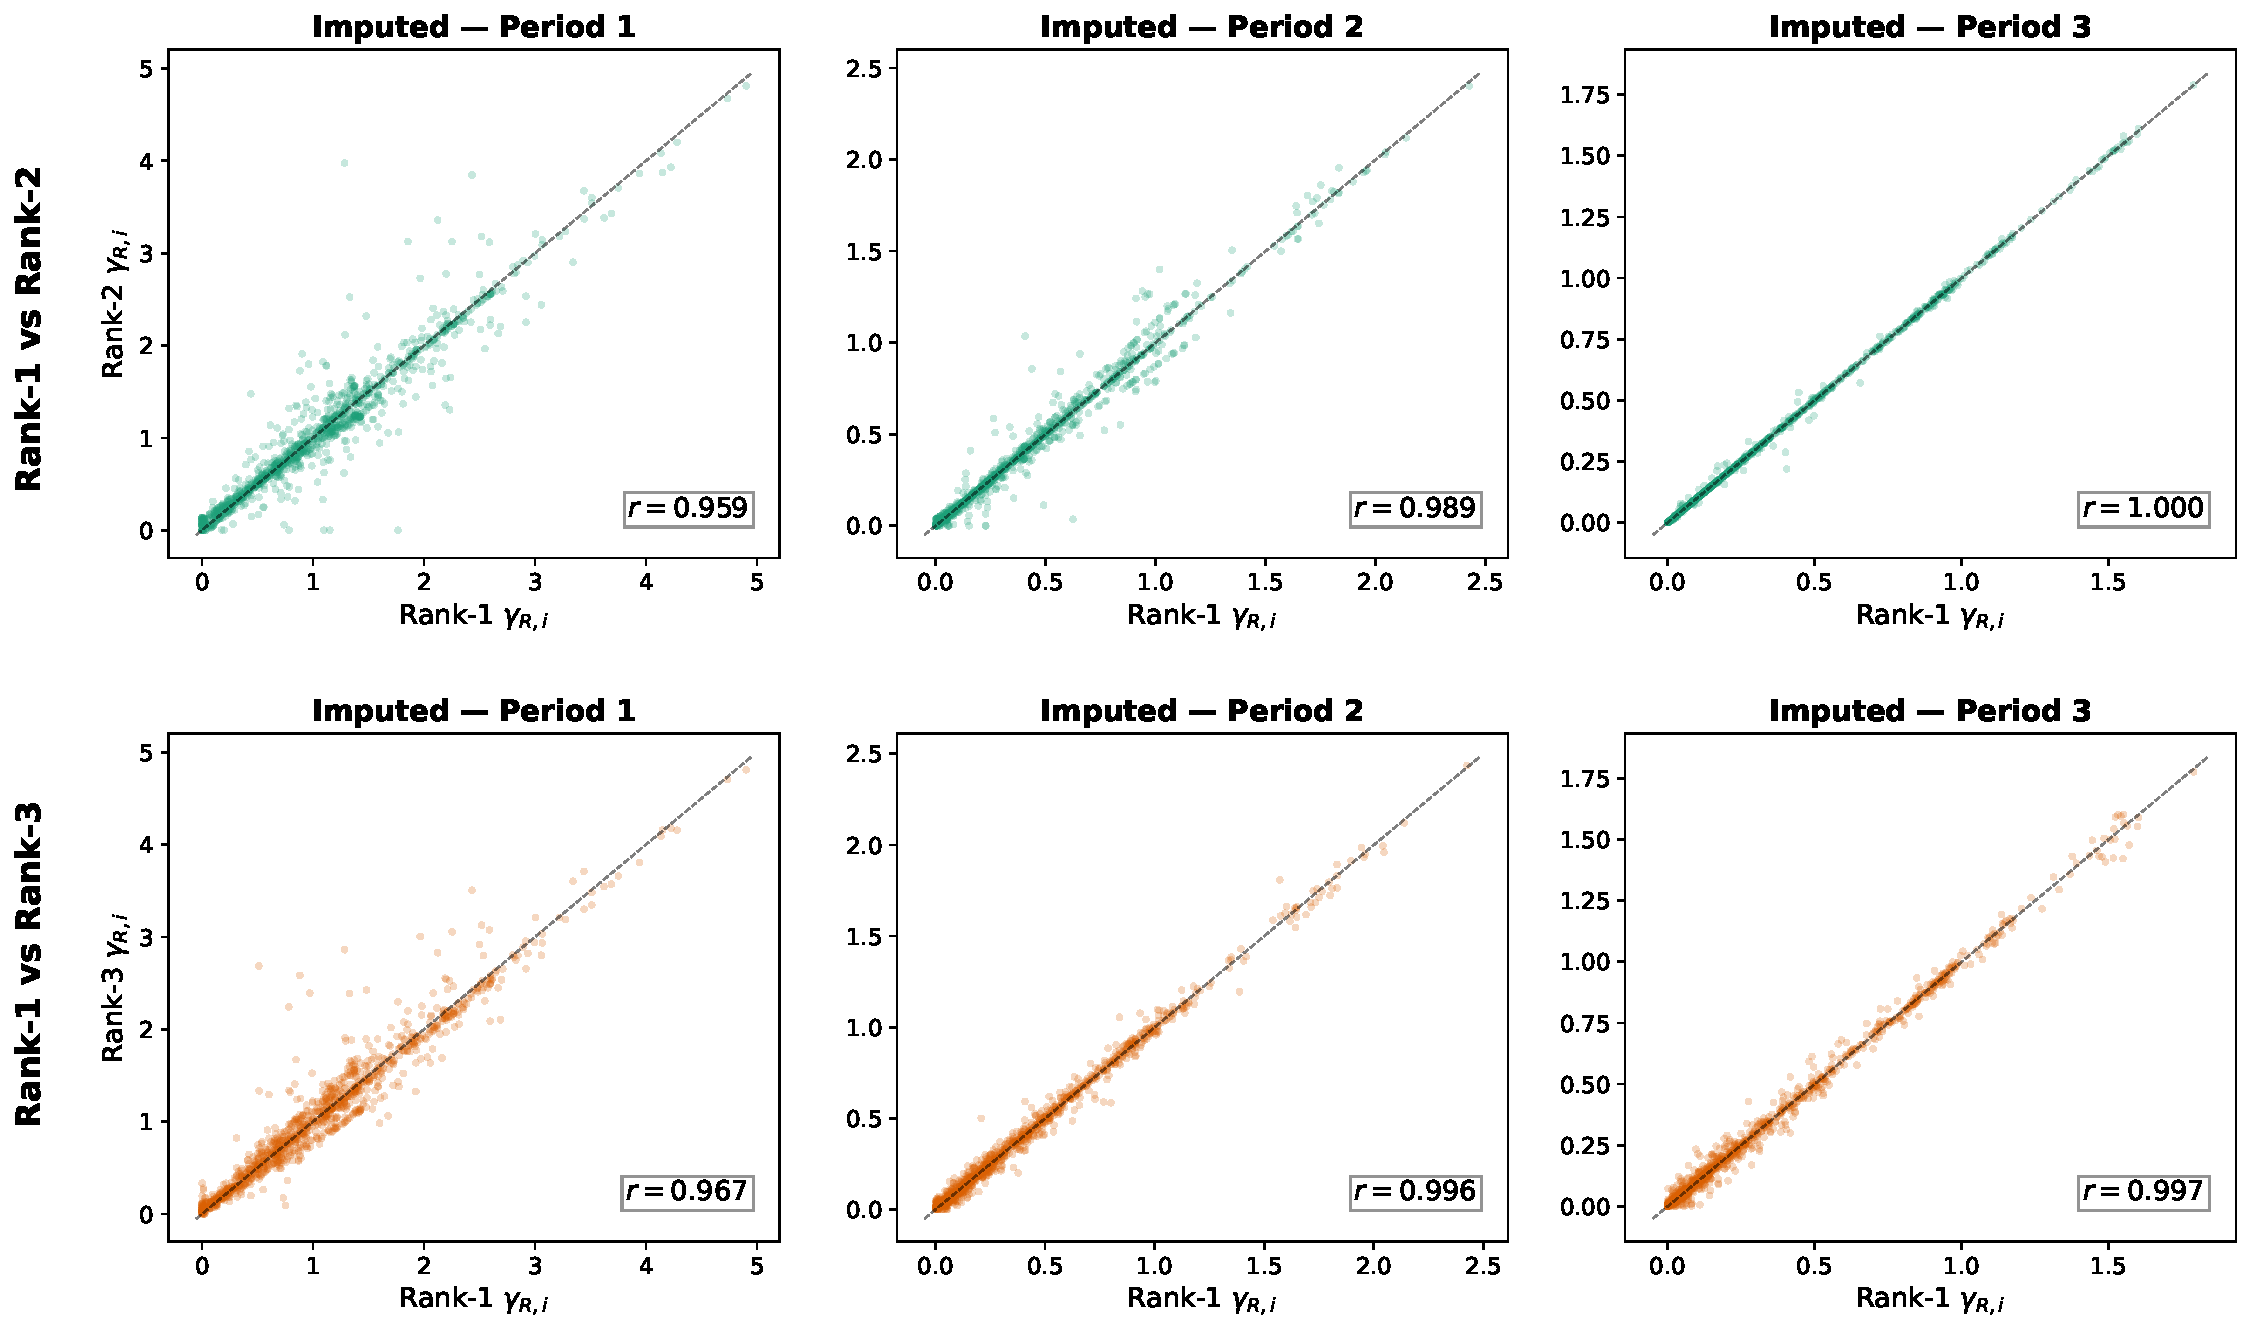
\includegraphics[width=\textwidth]{simulation_results/multiperiod_lowrank/scatter_rank1_vs_rank2_rank3_combined.png}
\caption{Scatter plots of imputed $\gamma_{R,i}$ entries: rank-1 vs.\ rank-2 (row~1) and rank-1 vs.\ rank-3 (row~2) across three pandemic periods. High correlation confirms that higher-rank models largely agree with the rank-1 baseline on unobserved policy-region combinations.}
\label{fig:rank1_vs_rank3_scatter_app}
\end{figure}

The scatter plots show high correlation between the rank-1 model and both higher-rank alternatives on imputed entries across all periods, confirming that the rank-1 separability assumption produces similar counterfactual estimates as more flexible models.

\subsection*{Alternative Specifications}

We also compare the rank-1 model against two natural baselines that each capture only one dimension of heterogeneity: (i) a \textbf{policy-only} model $\gamma_{R,i} = \beta_i$ that ignores region heterogeneity, and (ii) a \textbf{region-only} model $\gamma_{R,i} = \alpha_R$ that ignores policy heterogeneity. Both are special cases of the rank-1 model.

\begin{table}[h!]
\centering
\begin{tabular}{|c|c|c|c|}
\hline Model & 2020.03.15--2020.06.15 & 2020.06.15--2020.09.15 & 2020.09.15--2020.12.15\\\hline
Rank-1 & $\mathbf{0.378} \pm 0.042$ & $\mathbf{0.287} \pm 0.026$ & $0.296 \pm 0.019$ \\
Policy-only ($\beta_i$) & $0.402 \pm 0.036$ & $0.334 \pm 0.030$ & $0.291 \pm 0.023$ \\
Region-only ($\alpha_R$) & $0.511 \pm 0.056$ & $0.387 \pm 0.050$ & $0.292 \pm 0.038$ \\\hline
\end{tabular}
\caption{Holdout RMSE (mean $\pm$ std.\ over 20 random splits) for three model specifications across three pandemic periods (20\% held out). The rank-1 model outperforms both baselines in Periods~1 and~2; all models converge in Period~3.}
\label{tab:alt_specs_app}
\end{table}

The rank-1 model substantially outperforms both baselines in the first two periods, confirming that the multiplicative region--policy interaction captures real structure in the data. In Period~3, all three models converge to similar RMSE due to lower variance in the later pandemic phase.

\subsection*{Conclusion}

The multi-period holdout analysis demonstrates that the separability structure $\gamma_{R,i} = k_R g_i$ captures the essential structure in the region--policy interaction matrix across different phases of the pandemic. The rank-1 model achieves holdout RMSE comparable to or better than higher-rank alternatives, and outperforms simpler baselines that capture only one dimension of heterogeneity. This provides strong evidence that the rank-1 structure is a well-supported and parsimonious approximation for the purposes of counterfactual policy simulation.

\section{Sensitivity Analysis for Unmeasured Confounding}
\label{app:confounding}

A fundamental concern in any observational study of NPI effectiveness is the potential for unmeasured confounding. Because $\gamma_{R,i}$ is estimated by averaging the fitted $\gamma_R(t)$ curve over days when policy $i$ was active, the estimate may conflate the true causal effect of the NPI with concurrent changes in voluntary behavior, seasonal effects, testing capacity, and other unobserved factors. In this section, we provide two complementary analyses to quantify the robustness of our conclusions to plausible levels of confounding.

\subsection*{Approach 1: Policy Ranking Stability Under Confounding Perturbation}

Following the logic of \citeapp{cinelli2020making}, we design a sensitivity analysis that directly tests the robustness of the full policy ranking to unmeasured confounding. We shrink all policy-specific $\gamma_{R,i}$ values toward their cross-policy mean $\bar{\gamma}_R$ by a fraction $f \in [0,1]$:
\begin{equation}
    \gamma_{R,i}^{(f)} = (1-f)\,\gamma_{R,i} + f\,\bar{\gamma}_R, \qquad \bar{\gamma}_R = \frac{1}{|\mathcal{I}|}\sum_{i\in\mathcal{I}} \gamma_{R,i}. \label{eq:confounding_blend}
\end{equation}
At $f=0$, the original estimates are used. At $f=1$, all policies share an identical $\gamma$ (i.e., NPIs have no differential effect). This formulation targets the \emph{contrast} between policies rather than the absolute level of $\gamma$, making it invariant to the baseline transmission environment of each region.

For each value of $f$, we re-simulate all $6^3 = 216$ hypothetical policy sequences through the full THEMIS pipeline and record the resulting cost ranking. We compare the perturbed ranking to the baseline ($f=0$) ranking using the Spearman rank correlation coefficient $\rho$ and the top-$K$ overlap (the fraction of the $K$ lowest-cost policies at baseline that remain in the top-$K$ set under perturbation).

\subsection*{Approach 2: Event-Study Falsification Test}

We conduct an event-study regression at each of the policy transition events observed across all regions during March--July 2020. At each transition date $t_0$, we estimate:
\begin{equation}
    \gamma(t) = \alpha + \beta_{\text{post}} \cdot \mathbf{1}[t \geq t_0] + \beta_{\text{trend}} \cdot (t - t_0) + \varepsilon_t \label{eq:event_study}
\end{equation}
in a symmetric window around $t_0$. The coefficient $\beta_{\text{post}}$ captures the discrete jump in $\gamma$ at the policy transition, controlling for the local linear trend. If $\gamma$ merely follows a smooth trajectory unrelated to NPI timing, $\beta_{\text{post}}$ should be indistinguishable from zero. We test a directional prediction: when policies tighten (severity increases), $\gamma$ should decrease ($\beta_{\text{post}} < 0$); when policies relax, $\beta_{\text{post}} > 0$. We assess concordance using a binomial sign test and one-sample $t$-tests.

\section{Sensitivity to Granular Policy Partition}
\label{app:granular}

A potential concern---raised by Reviewer~1 and highlighted by the AE---is whether the 7-category MECE policy partition used in the main paper might obscure heterogeneity among individual NPI components, effectively assuming that sub-interventions within a category have additive or interchangeable effects. In this section, we demonstrate that refining the partition into a more granular set of categories does not fundamentally change the model's predictions or qualitative conclusions.

\subsection*{Construction of the Granular Partition}

The original 7 categories are constructed from binarized OxCGRT indicators via two composite features: \emph{Restrict Mass Gatherings} $= \mathbf{1}[\text{C3} \lor \text{C4} \lor \text{C5}]$ and \emph{Others} $= \mathbf{1}[\text{C2} \lor \text{C7} \lor \text{C8} \lor \text{H1}]$. To test sensitivity, we construct a finer partition that introduces \emph{within-category} variation based on the \textbf{overall OxCGRT stringency} (defined as $S = \sum_{k=1}^{8} \text{C}k_{\text{raw}}$, the sum of raw severity levels before flag-based binarization). For each of the four largest original categories, we split at the global median stringency into ``Moderate'' ($S \leq$ cutoff) and ``Strict'' ($S >$ cutoff) sub-categories. The three smallest categories (No Measure, Restrict Mass Gatherings, MG + Schools) have too few global observations to support a meaningful split and are retained as-is.

This yields 11 granular MECE categories, each a strict refinement of one of the original 7 categories. The mapping is detailed in Table~\ref{tab:granular_partition_app}.

\begin{table}[H]
\centering
\small
\begin{tabular}{|c|l|l|c|c|}
\hline
\textbf{ID} & \textbf{Granular Category} & \textbf{Original Category} & \textbf{Cutoff} & \textbf{Regions Obs.} \\\hline
G1 & No Measure & No Measure & --- & 89 \\
G2 & Restrict Mass Gatherings & Restrict Mass Gath.\ & --- & 0 \\
G3 & MG + Schools & MG + Schools & --- & 6 \\
G4 & Others Only -- Moderate & Others Only & $\leq 5$ & 80 \\
G5 & Others Only -- Strict & Others Only & $> 5$ & 64 \\
G6 & MG + Others -- Moderate & MG + Others (no Schools) & $\leq 11$ & 28 \\
G7 & MG + Others -- Strict & MG + Others (no Schools) & $> 11$ & 36 \\
G8 & MG + Schools + Others -- Moderate & MG + Schools + Others & $\leq 16$ & 89 \\
G9 & MG + Schools + Others -- Strict & MG + Schools + Others & $> 16$ & 121 \\
G10 & Lockdown -- Moderate & Lockdown & $\leq 20$ & 109 \\
G11 & Lockdown -- Strict & Lockdown & $> 20$ & 49 \\\hline
\end{tabular}
\caption{The 11 granular MECE policy categories, their mapping to the original 7 categories, the stringency cutoff used for the Moderate/Strict split, and the number of regions (out of 210) in which each was observed for $\geq$10 days during March--July 2020.}
\label{tab:granular_partition_app}
\end{table}

\subsection*{Rank-1 Holdout Analysis on the Granular Matrix}

We assemble the $210 \times 11$ partially-observed $\gamma_{R,i}$ matrix for the granular partition and repeat the holdout RMSE test from Appendix~\ref{app:separability}. The observation density is 29.0\% (compared to 47.3\% for the original $210 \times 7$ matrix), reflecting the sparser coverage of finer categories. The rank-1 model continues to achieve the lowest holdout RMSE:

\begin{table}[H]
\centering
\begin{tabular}{|c|cc|}
\hline
& \multicolumn{2}{c|}{Holdout RMSE (mean $\pm$ std)} \\
Rank $l$ & Original (7 categories) & Granular (11 categories) \\\hline
1 & $0.447 \pm 0.070$ & $0.464 \pm 0.055$ \\
2 & $0.552 \pm 0.046$ & $0.582 \pm 0.064$ \\
3 & $0.563 \pm 0.064$ & $0.596 \pm 0.059$ \\\hline
\end{tabular}
\caption{Holdout RMSE (20\% held out, 20 random splits) for rank-$l$ models under the original and granular policy partitions. The rank-1 model achieves the lowest RMSE in both cases, confirming the separability assumption.}
\label{tab:granular_rmse_app}
\end{table}

The rank-1 RMSE for the granular matrix ($0.464$) is close to the original ($0.447$), and higher-rank models perform worse---a clear overfitting signature. The separability structure $\gamma_{R,i} = k_R \gamma_i$ remains well-supported under the finer partition.

\subsection*{Prediction Comparison}

Using the granular $\gamma_{R,i}$ estimates, we re-run DELPHI for the four paper regions under their actual policy sequences during March 15--June 15, 2020. For each splittable category observed in a region, we compute the granular $\gamma$ by scaling the parent-category estimate proportionally to the mean stringency difference between the Moderate and Strict sub-categories, weighted by their respective observation counts. This ensures that the weighted average of sub-category gammas reproduces the parent gamma, while still allowing within-category variation to influence predictions. For unsplit or unobserved categories, we retain the parent estimate. The prediction comparison is shown in Figure~\ref{fig:granular_pred_app}.

\begin{figure}[H]
\centering
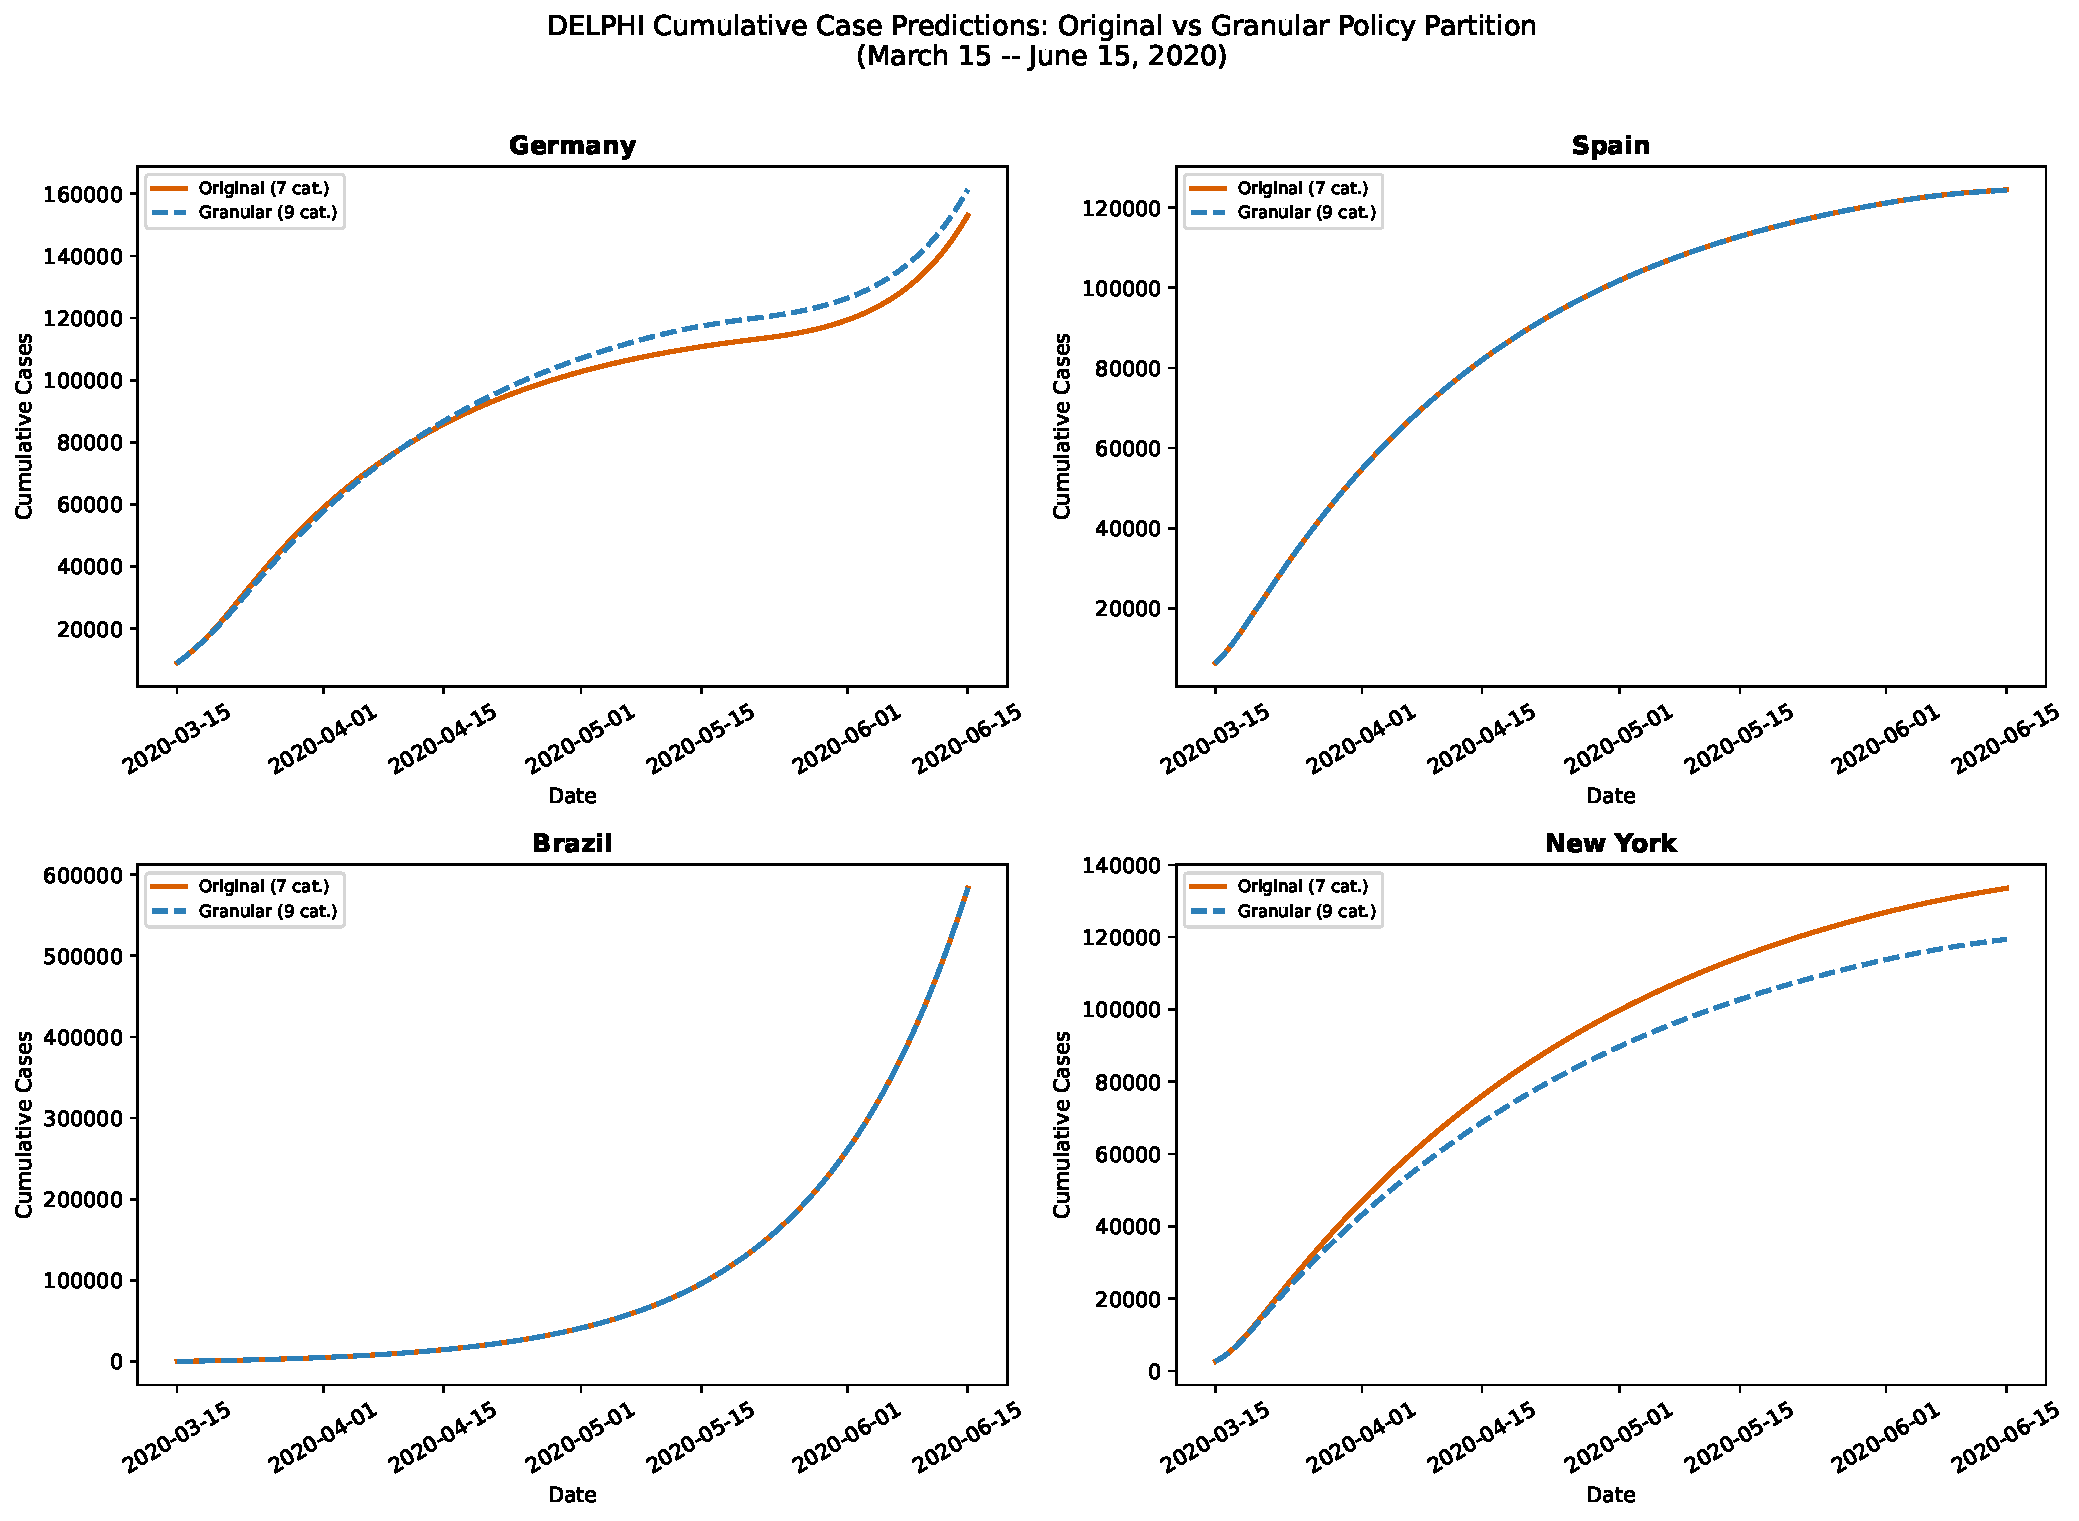
\includegraphics[width=\textwidth]{simulation_results/granular_policies/combined_prediction_comparison.png}
\caption{Cumulative case predictions under the original 7-category (solid orange) and granular 11-category (dashed blue) policy partitions for the March 15--June 15, 2020 period. The curves track closely in all regions with directionally consistent trajectories.}
\label{fig:granular_pred_app}
\end{figure}

The prediction differences are small across all regions: Germany (2.3\% cases, 2.1\% deaths), Spain (0.2\%, 0.1\%), Brazil (10.2\%, 10.1\%), and New York (0.2\%, 0.2\%). Brazil shows the largest deviation because it spent nearly its entire evaluation period under a single policy category (``Others Only''), so even the modest stringency-based adjustment compounds over 93 days of exponential dynamics. In contrast, Germany, Spain, and New York transition across multiple categories during the evaluation window, so sub-category adjustments partially offset each other. Importantly, both partitions agree on the direction of policy effects and preserve the qualitative ranking of policy sequences, confirming that the paper's conclusions are robust to within-category stringency heterogeneity.

\bibliographystyleapp{informs2014}
\bibliographyapp{Paper/bibliography.bib}
\end{APPENDICES}
\end{document}